\documentclass[11pt,a4paper]{article}

\usepackage{fontspec}
\usepackage{polyglossia}
\setmainlanguage{russian}
\setotherlanguage{english}
\setmainfont{PT Serif}[Ligatures=TeX]
\setsansfont{PT Sans}[Ligatures=TeX]
\setmonofont{PT Mono}[Scale=0.92]

% macOS ставит ParaType как .ttc, и fontconfig не рапортует покрытие кириллицы;
% polyglossia верит fontconfig и отказывается принимать основной шрифт, хотя
% кириллица в нём есть (проверено отдельной сборкой). Объявляем семейства явно ---
% это штатный обход, рекомендованный самим polyglossia, и на Linux он безвреден.
\newfontfamily\cyrillicfont{PT Serif}[Ligatures=TeX]
\newfontfamily\cyrillicfontsf{PT Sans}[Ligatures=TeX]
\newfontfamily\cyrillicfonttt{PT Mono}[Scale=0.92]

\usepackage{amsmath,amssymb}
\usepackage{graphicx}
\usepackage{booktabs}
\usepackage{tabularx}
\usepackage[table]{xcolor}
\usepackage[margin=27mm,top=25mm,bottom=27mm]{geometry}
\usepackage{caption}
\usepackage{enumitem}
\usepackage{hyperref}
\usepackage{microtype}

\captionsetup{font=small,labelfont=bf,labelsep=period,justification=justified}
\captionsetup[table]{skip=4pt}
\setlist{itemsep=2pt,parsep=0pt,topsep=4pt}
\hypersetup{colorlinks=true,linkcolor=black,urlcolor=black,citecolor=black,
            pdftitle={Модель предсказания ингибирования цитохромов P450},
            pdfauthor={команда CYP}}

\emergencystretch=2.2em
\setlength{\parskip}{0pt}
\setlength{\parindent}{1.2em}
\linespread{1.06}
\renewcommand{\arraystretch}{1.12}

\newcommand{\pic}{\mathrm{pIC}_{50}}
\newcommand{\pC}{\mathrm{p}C}
\newcommand{\Var}{\mathrm{Var}}
\newcommand{\E}{\mathbb{E}}

\title{\vspace{-14mm}\textbf{\Large Модель предсказания ингибирования цитохромов P450}\\[3mm]
\normalsize Устройство решения для OpenADMET CYP Blind Challenge: что в данных,\\
что мы измерили, как устроена модель и почему именно так}
\author{}
\date{\normalsize 27 августа 2026}

\begin{document}
\maketitle
\thispagestyle{empty}
\begin{abstract}
\noindent
Документ описывает решение задачи предсказания ингибирования четырёх изоформ цитохрома P450 по структуре
молекулы. Содержит разбор того, что лежит в данных и что мы из них измерили, устройство модели и обоснование
каждого её элемента, протокол проверки и список того, что уже проверено и не работает. Все числа получены
прогонами на открытых данных соревнования и воспроизводимы; графики построены по тем же прогонам.
Рассчитан на две аудитории сразу: на химика, знакомого с основами машинного обучения, и на специалиста
по машинному обучению, знакомого с основами биохимии.
\end{abstract}
\vspace{4mm}
{\small\tableofcontents}
\clearpage
\section{Задача}
\label{sec:task}

Вход --- SMILES молекулы. Оцениваемых треков два: регрессия и классификация. Третий, предсказание позы
лиганда в кармане фермента, откроется в середине соревнования и здесь не разбирается.

В регрессионном треке нужно выдать матрицу $\hat{Y} \in \mathbb{R}^{750\times 4}$: $\pic$ прямого
ингибирования для CYP1A2, CYP2C9, CYP2D6 и CYP3A4. В классификационном --- $\hat{Y} \in \{0,1\}^{750\times 2}$:
метку time-dependent ингибирования для 3A4 и 2D6. Тестовые 750 соединений выданы без меток, отправка
закрывается 3 ноября.

\subsection{Метрика регрессии и что из неё следует}

Метрика --- не средняя абсолютная ошибка. Организаторы публикуют вместе с каждым $\pic$ границы
доверительного интервала байесовской подгонки кривой, и ошибка считается до ближайшей границы, а не до
точечной оценки:
\begin{equation}
\text{ST-RAE} \;=\;
\frac{\sum_i \bigl[(\hat y_i - h_i)_+ + (l_i - \hat y_i)_+\bigr]}
     {\sum_i \bigl[(\bar y - h_i)_+ + (l_i - \bar y)_+\bigr]},
\qquad \bar y = \frac{1}{n}\sum_i y_i .
\label{eq:strae}
\end{equation}

Здесь $l_i$ и $h_i$ --- нижняя и верхняя границы интервала $i$-го соединения, а $(\cdot)_+ = \max(\cdot, 0)$.
Числитель: предсказание, попавшее внутрь полосы, не штрафуется вовсе, а вышедшее наружу штрафуется только
на расстояние до ближайшего края. Знаменатель: та же величина для константного предсказателя, выдающего
среднее по оценочному набору. Отношение единица означает, что модель не лучше предсказания одного числа для всех соединений подряд;
меньше единицы --- лучше.

Из этого следует три вещи, и каждая влияет на архитектуру.

Первое. Задача интервально-цензурированная, и обучаться надо на той же клипованной L1, а не на квадратичной
ошибке. Квадратичная будет тянуть предсказание к центру полосы там, где метрике всё равно, где именно
внутри полосы оно стоит.

Второе. Это отношение сумм, а не среднее отношений. Соединения с широкой полосой почти невесомы в обеих
частях: они дают мало и в числитель, и в знаменатель. Метрику определяют соединения с узкой полосой,
то есть активные, у которых кривая хорошо определена.

Третье. Оптимальная точечная оценка под \eqref{eq:strae} не обязана совпадать с условным средним
предсказательного распределения. Это разбирается в разделе~\ref{sec:decision}.

Знаменатель считается по среднему \emph{того набора}, на котором метрика вычисляется. У нас это среднее
по обучающей подвыборке фермента, на лидерборде --- по 750 тестовым соединениям. Значит наши числа и числа
лидерборда напрямую несопоставимы, даже если модель одна и та же; сопоставимы только разности между
вариантами, посчитанные на одном наборе.

\subsection{Метрика классификации}

Для TDI считается коэффициент корреляции Мэтьюса:
\begin{equation}
\text{MCC} = \frac{TP\cdot TN - FP\cdot FN}{\sqrt{(TP+FP)(TP+FN)(TN+FP)(TN+FN)}} .
\label{eq:mcc}
\end{equation}

Это коэффициент корреляции Пирсона между двумя бинарными векторами, предсказанным и истинным. При
несбалансированных классах он ведёт себя куда честнее точности: предсказать всем «нет» даёт точность
78 процентов и MCC ровно ноль.

MCC не раскладывается по объектам. Вклад одного соединения зависит от того, что
предсказано остальным, потому что все четыре счётчика стоят под общим корнем. Отсюда следует, что порог
0.5 почти никогда не оптимален и его надо выбирать явно --- см. раздел~\ref{sec:decision}.

Обе метрики агрегируются макро-усреднением по эндпойнтам, и лидерборд сортируется по этому среднему.
Организаторы пересчитывают его на 1000 бутстрап-выборках.

\section{Биохимия задачи}
\label{sec:bio}

Раздел для тех, кто пришёл со стороны машинного обучения: что физически стоит за каждой колонкой
в данных. Без этого половина решений в модели выглядит произволом.

\subsection{Что такое цитохромы P450 и почему именно эти четыре}

Цитохромы P450 --- надсемейство гем-тиолатных монооксигеназ. Гем --- порфириновое кольцо с железом
в центре, то же самое, что в гемоглобине; «тиолатные» означает, что пятое координационное место железа
занимает атом серы остатка цистеина. Название историческое: восстановленный комплекс фермента с угарным
газом даёт полосу поглощения при 450 нм.

Каталитический цикл в общем виде: фермент связывает субстрат, железо восстанавливается, присоединяет
кислород, кислород расщепляется с образованием высокореакционного оксоферрильного интермедиата
(Compound~I), который вырывает водород у субстрата и вставляет туда гидроксил. Суммарно
\[
\text{RH} + \text{O}_2 + \text{NADPH} + \text{H}^+ \;\longrightarrow\;
\text{ROH} + \text{H}_2\text{O} + \text{NADP}^+ .
\]
Электроны поставляет НАДФН через флавопротеин цитохром-P450-редуктазу. Для эксперимента отсюда следует вот что: без НАДФН фермент не работает, так что катализ можно включать
и выключать в пробирке. На этом приёме построено измерение TDI.

Смысл реакции --- сделать липофильную чужеродную молекулу более полярной, чтобы её можно было
конъюгировать (вторая фаза метаболизма) и вывести. Печёночные P450 --- главный барьер между
проглоченным веществом и системным кровотоком.

Изоформ у человека около 57, но лекарственный метаболизм сосредоточен в немногих. CYP3A4 отвечает
примерно за половину всех оборотов, CYP2D6, CYP2C9, CYP2C19 и CYP1A2 --- за большую часть остального.
Четвёрка в соревновании покрывает подавляющее большинство клинически значимых взаимодействий.

\subsection{Почему ингибирование --- проблема}

Если препарат A ингибирует фермент, который выводит препарат B, концентрация B в крови растёт ---
иногда в разы. Для препарата с узким терапевтическим окном это прямая дорога к токсичности, вплоть
до снятия с рынка уже зарегистрированного средства, безопасного само по себе.

Поэтому ингибирование P450 проверяют рано, ещё на стадии выбора соединения-кандидата. Предсказание
по структуре экономит эти пробы, и цена ошибки здесь измеряется в снятых с разработки молекулах.

\subsection{Что такое IC$_{50}$ и pIC$_{50}$}

В пробу вносят фермент, зонд-субстрат с известной скоростью превращения и испытуемое соединение
в нескольких концентрациях. Измеряют, насколько упала скорость превращения зонда. IC$_{50}$ ---
концентрация испытуемого соединения, при которой скорость падает вдвое. $\pic = -\log_{10}$IC$_{50}$
в молях на литр: $\pic = 6$ соответствует одному микромолю, $\pic = 4$ --- ста микромолям. Больше $\pic$ ---
сильнее ингибитор.

Важная оговорка: IC$_{50}$ --- не константа связывания. Она зависит от концентрации зонд-субстрата
и от механизма (конкурентный ингибитор вытесняется субстратом, неконкурентный --- нет); связь
с константой ингибирования $K_i$ даёт соотношение Ченга--Прусоффа. Сравнивать IC$_{50}$ между
лабораториями и пробами напрямую нельзя, внутри одного набора --- можно, и именно это мы и делаем.

\subsection{Как читают результат и откуда берутся артефакты}

Зонд-субстрат подбирают так, чтобы его превращение было легко измерить. Способов два.

\emph{Флуоресцентный}: зонд после окисления даёт флуоресцирующий продукт, и прибор просто меряет
свечение. Дёшево и быстро, поэтому так сделаны 1A2, 2C9 и 3A4 в этом наборе.

\emph{Масс-спектрометрический}: продукт детектируют по массе. Дороже, но специфичнее; так сделан 2D6.

Отсюда конкретный артефакт. Если испытуемое соединение само флуоресцирует в том же диапазоне или,
наоборот, тушит флуоресценцию продукта, прибор покажет изменение сигнала, которого химически не было.
Ложное «ингибирование» появится в трёх флуоресцентных эндпойнтах и не появится в масс-спектрометрическом.
Поэтому в модели заведён отдельный канал артефактов пробы (раздел~\ref{sec:artifact}): это конфаундер с известной
структурой, а не шум.

\subsection{Что такое time-dependent ингибирование}
\label{sec:tdi}

Обычное ингибирование обратимо: молекула садится в карман, мешает субстрату, отпускает. Уберите
ингибитор --- активность вернётся.

Time-dependent ингибирование, оно же механизм-зависимая инактивация, устроено иначе. Фермент сам
превращает соединение в реакционноспособный продукт, и этот продукт остаётся --- ковалентно
модифицирует гем или белок, либо образует прочный комплекс с железом (metabolite-intermediate complex).
Фермент выведен из строя необратимо. Отличительные признаки: процесс требует катализа (без НАДФН
не идёт), развивается во времени, насыщается по концентрации, и активность не восстанавливается
отмывкой.

Клинически это гораздо хуже обратимого ингибирования. Обратимый ингибитор перестаёт мешать, как только
выводится из организма. Инактивированный фермент восстанавливается только синтезом нового белка,
а на это уходят сутки-двое. Поэтому эффект накапливается при повторных приёмах и держится долго после
отмены.

\paragraph{Как это измеряют.} Ставят два плеча одной пробы.

\emph{Прямое плечо}: соединение и зонд-субстрат вносят одновременно, сразу меряют IC$_{50}$. Видно
обратимое ингибирование.

\emph{Плечо с преинкубацией}: соединение сначала выдерживают с ферментом и НАДФН, дав катализу
поработать, и только потом вносят зонд и меряют IC$_{50}$. Если соединение --- механизм-зависимый
инактиватор, за время преинкубации часть фермента выведена из строя, и измеренная IC$_{50}$ окажется
ниже: соединение выглядит потентнее, чем было.

Разница между плечами и есть сигнал. В логарифмической шкале это сдвиг
\[
\Delta = \pi_{\text{после преинкубации}} - \pi_{\text{прямое}} \;\ge\; 0 ,
\]
и неотрицательность здесь не соглашение, а физика: преинкубация может только добавить инактивации,
но не отменить обратимое связывание. Двукратный сдвиг IC$_{50}$ --- то есть $\Delta > \log_{10}2 \approx 0.301$
--- общепринятый порог, за которым соединение помечают как TDI.

Отсюда становится понятной вторая ветвь правила разметки из раздела~\ref{sec:decision}. Соединение может
быть настолько слабым обратимым ингибитором, что в прямом плече его IC$_{50}$ вообще не определяется
как значимая ($\pi \le 4$, то есть слабее ста микромолей). Но если после преинкубации оно перешло порог
активности с тем же двукратным запасом ($\pi + \Delta > 4 + \log_{10}2$), это тоже TDI --- просто
инактивация оказалась единственным его механизмом. Правило и состоит из этих двух случаев.

\subsection{Что такое Emax и положительный контроль}

Кривая доза-эффект выходит на плато. Высота плато --- Emax, предельная доля подавленной активности.
Полный ингибитор обнуляет активность, частичный оставляет какую-то долю сколь угодно высокой
концентрации. Причины частичности бывают разные: соединение садится не в каталитический карман,
а в аллостерический; или у фермента несколько сайтов связывания субстрата, как у CYP3A4.

Измеряют Emax не в абсолютных единицах, а относительно положительного контроля --- известного полного
ингибитора этого фермента, который ставят в ту же пробу. Отсюда шкала в данных: полный ингибитор даёт
примерно $-1$, потому что подавил столько же, сколько контроль. Такая нормировка снимает разброс между
планшетами и партиями фермента.

\subsection{Чем четыре фермента различаются}
\label{sec:isoforms}

Отсюда понятно, почему модель устроена как многозадачная с явной матрицей связей, а не как одна голова.

\emph{CYP3A4} --- самый крупный и самый неразборчивый. Активный карман большой и податливый, вмещает
молекулы вплоть до циклических пептидов; в нём помещается больше одного лиганда одновременно, откуда
кооперативность и не всегда сигмоидные кривые. Узнавание в основном гидрофобное, поэтому предсказатель
«крупная жирная молекула --- вероятный ингибитор» работает удивительно хорошо. Отсюда и лучшая
предсказуемость 3A4 в наших измерениях.

\emph{CYP2C9} --- карман поменьше, на входе положительно заряженный остаток аргинина, притягивающий
анионы. Субстраты преимущественно кислые, с карбоксильной или другой ионизуемой группой. С 3A4 частично
перекрывается по липофильности, отсюда ранговая корреляция 0.69.

\emph{CYP1A2} --- узкая плоская щель. Субстраты --- плоские ароматические системы, полициклика
и азотистые гетероциклы. Они же его и индуцируют, из-за чего у курильщиков клиренс некоторых препаратов
заметно выше.

\emph{CYP2D6} объясняет половину этого документа. В активном центре сидят остатки аспартата и глутамата,
дающие солевой мостик с протонированным атомом азота лиганда. Практически все известные субстраты
и ингибиторы 2D6 --- основания, заряженные при физиологическом pH. Узнавание идёт не по общей
липофильности, а по конкретному электростатическому взаимодействию на конкретном расстоянии
от ароматического ядра.

Долю протонированной формы даёт уравнение Гендерсона--Хассельбальха:
\begin{equation}
f_{\text{прот}} = \frac{1}{1 + 10^{\,\mathrm{pH} - \mathrm{p}K_a}} .
\label{eq:hh}
\end{equation}
При pH 7.4 третичный амин с $\mathrm{p}K_a$ около 9.8 заряжен на 99.6 процента, пиридиновый азот
с $\mathrm{p}K_a$ 5.2 --- на 0.6 процента, а амид не заряжен вовсе. Разница в сто с лишним раз
по доле заряженных молекул. Фингерпринт, считающий фрагменты в радиусе двух связей, видит во всех трёх
случаях просто «атом азота в таком-то окружении» и различить их не может --- отсюда механистический
блок признаков.

И ещё: 2D6 сильно полиморфен. Часть популяции несёт
неработающие аллели, часть --- дупликации гена; это делает предсказание ингибирования 2D6 клинически
особенно ценным, но на наши данные не влияет, поскольку измерения делаются на рекомбинантном ферменте
одного варианта.

\section{Данные}
\label{sec:data}

Пять таблиц, около 35 тысяч строк. Устройство этих данных важнее их объёма: вся конструкция модели вырастает из одной асимметрии.
Обучающая матрица разрежена и смещена отбором, тестовая плотная.

\begin{table}[htbp]\centering\small
\begin{tabularx}{\textwidth}{@{}Xllp{62mm}@{}}
\toprule
Источник & Форма & Заполнено & Что это \\
\midrule
Кривые доза-эффект, прямое плечо & $4905\times 4$ & 26--48\,\% & $\pic$ плюс границы интервала и стандартная ошибка \\
Кривые, плечо с преинкубацией & $6145\times 4$ & 21--58\,\% & то же для условия TDI \\
Emax, оба плеча & $6146\times 8$ & частично & предельная глубина подавления и её интервал \\
Одноточечный скрининг & $4376\times 4$ & 100\,\% & $\log_2$fc при 49.5 мкМ и стандартная ошибка \\
Тест & $750\times 4$ & --- & слепой, плотный \\
\bottomrule
\end{tabularx}
\caption{Пять источников. Пересечения между ферментами внутри таблицы кривых маленькие: одновременно
для 1A2 и 2C9 измерено 295 соединений, для 2C9 и 2D6 --- 230. Скрининг --- единственный плотный
источник, и он покрывает весь диапазон активностей, включая неактивные соединения, которых в кривых
почти нет.}
\end{table}

\subsection{Что меряют эти таблицы}

Кривая доза-эффект: соединение разводят по концентрациям, для каждой измеряют, насколько подавлена
активность фермента, и через полученные точки проводят сигмоиду. Из подгонки получают $\pic$ ---
отрицательный десятичный логарифм концентрации, при которой активность падает вдвое. Байесовская подгонка
даёт не только точку, но и интервал, отражающий, насколько уверенно эта точка определена. У соединений,
чья кривая не дошла до плато, интервал широкий.

Одноточечный скрининг: то же измерение, но при одной концентрации 49.5 мкМ. На выходе $\log_2$fc ---
логарифм отношения сигнала с соединением к сигналу без него. Ноль означает, что ничего не произошло,
отрицательные значения --- что активность подавлена.

Полные кривые снимали не для всех подряд. Соединение поднимали на подробное
измерение, если оно показало эффект на скрининге. Это отбор по зависимой переменной, и он деформирует
обучающую выборку способом, который разобран в разделе~\ref{sec:d6}.

Правило это не универсальное. Скрининг есть у 4375 из 4905 соединений с кривыми; у оставшихся 530 его
нет, и все 530 несут метку \emph{только} по 3A4 --- на 1A2, 2C9 и 2D6 у них меток ноль. То есть для трёх
ферментов отбор по скринингу описывает выборку целиком, а на 3A4 почти четверть кривых (530 из 2335)
пришла каким-то другим путём, и для них аргумент про отбор просто не про них.

\subsection{Как собран тестовый набор}

Организаторы описали процедуру: взяли по 25 лучших ингибиторов каждого из 1A2, 2C9 и 3A4, к каждому
добавили по 10 ближайших соседей по фингерпринту, итого $3\times 25\times 10 = 750$.

Это проверяется, и проверка сходится частично. Здесь важно, что порог кластеризации выбирается, а не
выводится, и картина от него зависит сильно. При рабочем пороге 0.35 из 750 тестовых соединений выходит
477 групп с медианным размером один, групп по пять и более членов 21, и в них лежат 155 соединений.
При 0.48 --- 203 группы с медианным размером два, 56 групп по пять и более, в них 496 соединений.
То есть серийная структура в наборе есть, но её видимый охват меняется от пятой части до двух третей
в зависимости от того, что считать серией. Ровно 75 серий ровно по 10 не восстанавливается ни при каком
пороге --- число 75 получается делением 750 на 10.

Что восстанавливается уверенно, так это положение якорей: оно от порога почти не зависит. Для каждой
группы найдено ближайшее обучающее соединение, и его активность стоит на 92--94 перцентиле обучающего
распределения по 1A2 и на 97.5--99 по 2C9 при любом пороге от 0.35 до 0.50, тогда как по 2D6, который
в отборе не участвовал, --- на 58--66. По 3A4 оценка гуляет заметно шире, от 82 до 95, и опирать на неё
точное число нельзя. Оговорка, без которой эти проценты читаются неверно: якорей с меткой всего от
девяти до тридцати семи на фермент, так что медиана здесь имеет широкий интервал. Медианное сходство
Танимото тестового соединения с ближайшим обучающим равно 0.587.

Значит распределение меток на тесте не совпадает с обучающим: тест обогащён активными по трём ферментам
и близок к фону по четвёртому. И устроен он как набор серий аналогов вокруг известных хитов, а не как
случайная выборка из химического пространства. Проверять модель надо соответственно.

\section{Что мы измерили до того, как что-то строить}

Первое, что было сделано --- простая базовая линия и разбор, почему она ведёт себя так, как ведёт.
Без этого нет способа отличить работающую конструкцию от красивой.

Базовая линия: счётчики фрагментов Моргана радиуса 2 (2048 бит), 217 дескрипторов RDKit, градиентный
бустинг, пятикратная кросс-валидация по кластерам Бутины при пороге сходства 0.35.

\begin{figure}[htbp]\centering
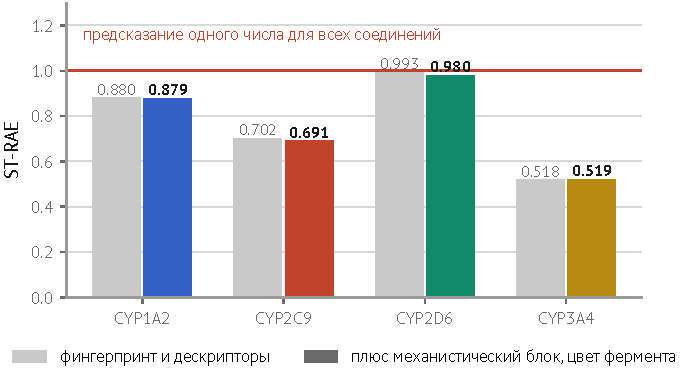
\includegraphics{fig/baseline}
\caption{Базовая линия регрессионного трека. Красная линия --- уровень предсказания одного числа
для всех соединений. CYP3A4 предсказывается вдвое лучше этого уровня, CYP2D6 --- на две сотых.}
\label{fig:baseline}
\end{figure}

Числа по ферментам: 1A2 --- ST-RAE 0.880 при Спирмене 0.497; 2C9 --- 0.702 и 0.583; 2D6 --- 0.993
и 0.351; 3A4 --- 0.518 и 0.764. Макро 0.773. Коэффициент детерминации на тех же фолдах: 0.216, 0.350,
0.122, 0.589.

CYP2D6 практически не предсказывается. Это и стало главным предметом разбирательства, потому что от
объяснения зависит, что вообще строить дальше.

\subsection{Версия первая: метки шумные, учить нечего}

Если почти весь разброс опубликованных активностей --- погрешность измерения, то потолок для любой модели
низкий и делать нечего. Обычно разделить настоящий разброс и шум трудно, но здесь вместе с каждым значением
опубликована его собственная стандартная ошибка.

Дисперсии независимых источников разброса складываются, поэтому
\begin{equation}
\Var(\text{наблюдаемое}) = \Var(\text{настоящее}) + \Var(\text{шум}),
\qquad
\text{надёжность} = 1 - \frac{\Var(\text{шум})}{\Var(\text{набл.})} .
\label{eq:rel}
\end{equation}

Надёжность --- доля разброса меток, которая приходится на настоящие химические различия. Она же задаёт
потолок $R^2$ для любой модели на этих метках: предсказать шум нельзя.

Для CYP2D6 стандартное отклонение меток 0.916, среднеквадратичная погрешность одного измерения 0.236,
надёжность 0.934. По остальным ферментам от 0.898 до 0.948. Версия не подтвердилась: сигнала в метках
достаточно. Сравнивая достигнутый $R^2$ с этим потолком, модель осваивает на 2D6 лишь восьмую часть
доступного ($0.122$ из $0.934$) и две трети на 3A4 ($0.589$ из $0.898$).

Оговорка, которую надо держать в голове. Слово «среднеквадратичная» здесь существенно: медианная
погрешность на 2D6 равна 0.069, то есть в три с половиной раза меньше, а почти шестьдесят процентов всей
шумовой дисперсии дают верхние пять процентов соединений с развалившейся подгонкой. В разложение
\eqref{eq:rel} идёт именно средний квадрат, так что число верное, но шум резко гетероскедастичен,
и взвешивание по индивидуальной погрешности важнее, чем кажется по среднему.

\subsection{Версия вторая: не хватает нужных признаков}

Как разобрано в разделе~\ref{sec:isoforms}, CYP2D6 узнаёт субстраты через солевой мостик
с протонированным азотом, а не через общую липофильность. Фингерпринт про заряд не знает: третичный амин
и амид для него --- два похожих азота в похожем окружении, хотя доля заряженной формы у них различается
в сотни раз.

Собрали блок из 28 химически осмысленных чисел: оценка $\mathrm{p}K_a$ самого основного центра, доля
протонированной формы при pH 7.4, полный заряд молекулы, счётчики классов азота и кислотных групп,
топологическое расстояние от заряженного азота до ближайшего ароматического кольца. Оценщик
$\mathrm{p}K_a$ --- правило: базовое значение класса минус индуктивный штраф от электроноакцепторных
заместителей с затуханием по числу связей. На двадцати соединениях с литературными значениями средняя
ошибка 0.60 единицы, медианная 0.2, и на бинарный вопрос «заряжено ли при 7.4» правило ответило верно
во всех двадцати случаях.

Результат двойственный, и это тот случай, когда полезно смотреть на две метрики сразу.

По ST-RAE выигрыша нет. Парный бутстрап по соединениям даёт для 2D6 разность $-0.012$ с интервалом
от $-0.041$ до $+0.017$; на макро-уровне $-0.0056$ с интервалом от $-0.0155$ до $+0.0041$. Интервалы
накрывают ноль.

По ранжированию выигрыш есть, и он избирателен именно так, как предсказывает химия. Спирмен на 2D6 растёт
с 0.351 до 0.403, разность $+0.052$ с интервалом от $+0.022$ до $+0.082$ и вероятностью отсутствия
прироста 0.001. На 2C9 $+0.014$ на грани значимости, на 1A2 и 3A4 нули с интервалами шириной в две сотых.

Ещё показательнее вот что: модель, построенная только на двадцати восьми механистических числах, без
фингерпринта и дескрипторов, воспроизводит на 2D6 92 процента ранжирующей способности модели на
фингерпринте с дескрипторами и 80 процентов от полной модели со всеми блоками --- против 43--53 процентов
на трёх остальных при любом из двух знаменателей. Сигнал CYP2D6 низкоразмерный и химически специфичный.

Итог: механизм назван верно, но выигрыш по метрике соревнования неотличим от нуля. Признаки --- часть
ответа, не главная его часть.

\subsection{Версия третья: дело в том, какие соединения попали в выборку}
\label{sec:d6}

\begin{figure}[htbp]\centering
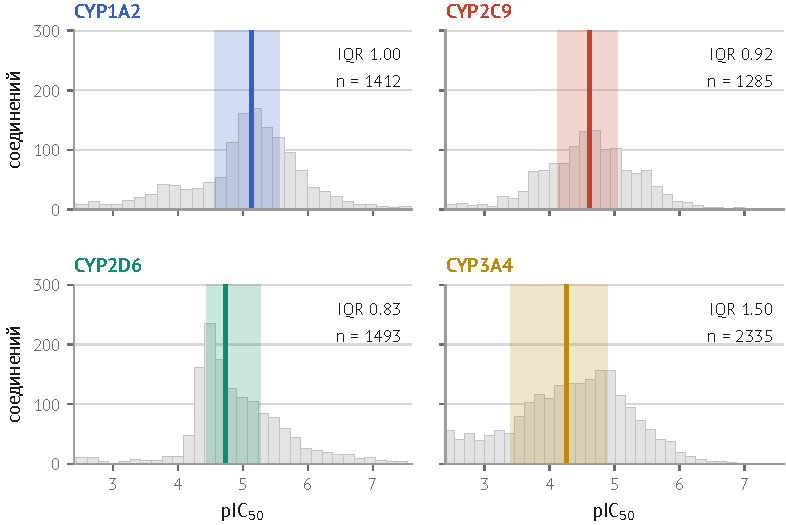
\includegraphics{fig/dists}
\caption{Распределения измеренных активностей. Цветом выделены средние 50 процентов соединений.
У CYP3A4 задача во многом сводится к тому, чтобы отделить левую часть от правой. У CYP2D6 левой части
почти нет, и модели приходится различать соединения внутри узкой полосы.}
\label{fig:dists}
\end{figure}

У CYP2D6 отбор оставил узкую полосу: средняя половина соединений уместилась в интервал шириной 0.83
логарифмической единицы против 1.50 у CYP3A4. Это ограничение диапазона, оно же selection
on the dependent variable: если отобрать объекты по интересующему признаку и потом мерить связь только
среди отобранных, связь ослабевает, хотя в полной популяции она никуда не делась.

Проверка требует второго показателя активности того же фермента, измеренного \emph{без} отбора. Он есть:
$\log_2$fc скрининга, снятый для 4375 соединений подряд, включая неактивные. Учим ту же модель на тех же
признаках и тех же фолдах предсказывать его вместо $\pic$.

Чтобы это не превратилось в сравнение «больше примеров против меньше», сделан контроль: из соединений
со скринингом случайно выбирается ровно столько же, сколько у этого фермента меток кривых.

\begin{figure}[htbp]\centering
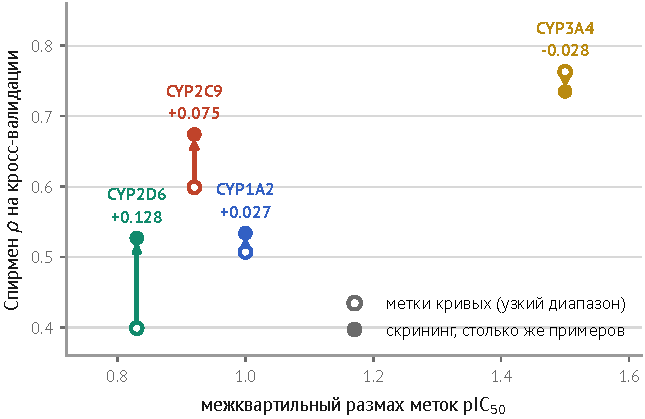
\includegraphics{fig/range}
\caption{Выигрыш от перехода на показатель с полным диапазоном против ширины полосы меток. Пустой кружок ---
качество на метках кривых, закрашенный --- на скрининге при равном числе обучающих примеров. Стрелка
тем длиннее, чем уже полоса меток, и на CYP3A4 разворачивается.}
\label{fig:range}
\end{figure}

Прирост монотонно падает с ростом размаха меток: 2D6 $+0.128$, 2C9 $+0.075$, 1A2 $+0.027$, 3A4 $-0.028$.
Четыре точки, монотонно, и отрицательный знак на CYP3A4 работает внутренним контролем против объяснения
«скрининг просто легче предсказуем сам по себе». На 2D6 при равном числе примеров $R^2$ поднимается
с 0.136 до 0.323.

Модель прекрасно умеет учить химию CYP2D6, но не может показать это на выданных метках. Основная причина
провала --- геометрия меток, и чинится она не признаками, а тем, что в правдоподобие входит источник
с полным диапазоном. На этом и построено всё остальное.

Честная оговорка про контроль: выровнено количество примеров, но не форма распределения меток. Совсем
чистый эксперимент требует подобрать подвыборку так, чтобы совпадало и то и другое.

\section{Порождающая модель}
\label{sec:gen}

Все пять таблиц --- наблюдения над одним объектом: кривой доза-эффект для тройки «молекула $m$,
фермент $e$, плечо $a$» (плечо --- прямое измерение или измерение после преинкубации). Модель
описывает эту кривую, а не отдельные таблицы, и каждая таблица подключается своим
правдоподобием.

Слово «правдоподобие» здесь ключевое и дальше встречается постоянно, поэтому стоит сказать,
что за ним стоит. Настоящей кривой мы не видим никогда --- видим только результаты измерений,
каждое со своим шумом. Правдоподобие отвечает на вопрос: если предположить, что настоящая
кривая вот такая, насколько ожидаемым было бы то, что мы на самом деле намерили? Обучение
состоит в переборе возможных кривых в пользу тех, при которых наблюдения выглядят наименее
удивительно. Записывают это обычно через $-\log p$ --- логарифм берут, чтобы вероятности
разных измерений складывались, а не перемножались, а минус --- чтобы задача стала задачей
минимизации. Ценность такой записи в том, что каждый источник данных добавляет в общую сумму
своё слагаемое, и разные по природе измерения оказываются на одном языке.

Латентные параметры тройки:
\begin{equation}
\theta_{m,e,a} = (\pi_{m,e,a},\; E_{m,e,a},\; h_e),
\qquad
\pi_{m,e,\text{tdi}} = \pi_{m,e,\text{dir}} + \Delta_{m,e} .
\label{eq:theta}
\end{equation}

Здесь $\pi$ --- потенция, та самая $\pic$; $E$ --- предельная глубина подавления, то есть какая доля
активности фермента подавляется при бесконечной концентрации; $h$ --- крутизна перехода, вынесенная
на уровень фермента (почему --- в разделе~\ref{sec:ident}).

Сдвиг $\Delta$ по химии неотрицателен: преинкубация может только усилить ингибирование, а не
ослабить. В данных предпосылка выполняется, и всё же \emph{ограничение не накладывается}. Жёсткое
$\Delta \ge 0$ доведено до кода и измерено на четырёх разбиениях: ранг падает на всех четырёх
ферментах, тогда как та же вторая голова без ограничения нейтральна. Прежняя редакция несла
неравенство прямо в определении \eqref{eq:theta}; оно оттуда убрано, потому что это не свойство
модели, а гипотеза, которая проверена и отвергнута. Разбор --- в разделе~\ref{sec:neg}.

Прямая модель прибора --- доля подавленной активности при концентрации $C$:
\begin{equation}
I(C;\theta) = \frac{E}{1 + 10^{\,h(\pC - \pi)}},
\qquad \pC = -\log_{10} C .
\label{eq:hill}
\end{equation}

Уравнение Хилла. При $\pC = \pi$, то есть когда концентрация равна IC$_{50}$, показатель обнуляется
и подавлена ровно половина от предельной глубины. Выше концентрация --- меньше $\pC$ --- отрицательнее
показатель --- ближе $I$ к $E$. Ниже --- наоборот. Крутизна $h$ задаёт, за сколько декад концентрации
происходит переход: при $h = 1$ путь от десяти до девяноста процентов эффекта занимает примерно две декады.

\subsection{Правдоподобия по источникам}

Кривая из двенадцати точек даёт несимметричную оценку: интервал вокруг $\pic$ обычно длиннее с одной
стороны. Усреднять границы --- терять эту информацию, поэтому порождающая модель задаёт расщеплённую нормаль с двумя
масштабами:
\begin{equation}
-\log p(y_{\text{крив}} \mid \pi)
= \operatorname{split-}\!\mathcal{N}(\pi;\, \hat\pi,\, \sigma^-,\, \sigma^+),
\qquad
\sigma^- = \frac{\hat\pi - l}{1.96},\quad \sigma^+ = \frac{h - \hat\pi}{1.96} .
\label{eq:split}
\end{equation}

Две половинки нормального распределения с разными ширинами, сшитые в моде и отнормированные общим
множителем $2/[\sqrt{2\pi}(\sigma^-+\sigma^+)]$. Правило деления на 1.96 точно только при симметричной
полосе: у расщеплённой нормали слева лежит масса $\sigma^-/(\sigma^-+\sigma^+)$, а не половина, поэтому
квантиль стоит не в 1.96 сигмы. На наших данных полосы почти симметричны --- максимум медианной асимметрии
0.13 логарифмической единицы --- и расхождение составляет 0.0004 единицы $\pic$. Правило годится, но
по этой причине, а не по общей верности.

\emph{И вся эта спецификация измерена, и она проигрывает.} Расщеплённая нормаль как обучающая цель
доведена до кода и прогнана на четырёх разбиениях против квадратичной потери, в двух углах: сама по
себе и поверх мёртвой зоны раздела~\ref{sec:deadzone}.

\begin{center}
\begin{tabular}{lcc}
\toprule
цель & ST-RAE & ранг \\
\midrule
квадратичная                    & 0.7204 & 0.5615 \\
расщеплённая нормаль            & 0.8106 & 0.5098 \\
квадратичная + мёртвая зона     & 0.6835 & 0.5955 \\
расщеплённая нормаль + мёртвая зона & 0.7252 & 0.5680 \\
\bottomrule
\end{tabular}
\end{center}

$-0.0517$ ранга сама по себе, минус на всех четырёх ферментах, и $-0.0275$ поверх мёртвой зоны. Два
угла нужны были потому, что одно сравнение с квадратичной не отличило бы «помогает асимметрия» от
«помогает полоса», --- и ответ ни то ни другое: жёсткий допуск несёт информацию полосы целиком, а
градуированный вес не добавляет к нему ничего и сам по себе отнимает.

Описание данных при этом верное: полосы действительно асимметричны, и усреднение границ действительно
теряет информацию. Неверным оказался переход от описания к обучающей цели.

Скрининг входит через \eqref{eq:hill} с аффинной калибровкой на фермент:
\begin{equation}
\hat y_{\text{скр}} = s_e \cdot \log_2\bigl(1 - I(C_0;\theta_{\text{dir}})\bigr) + b_e,
\qquad
-\log p(y_{\text{скр}} \mid \theta,\psi_e)
= \frac{(y_{\text{скр}} - \hat y_{\text{скр}})^2}{2(\sigma_i^2 + \sigma_e^2)} + \log\sqrt{\sigma_i^2+\sigma_e^2}.
\label{eq:scr}
\end{equation}

Прибор показывает логарифм оставшейся активности, отсюда $\log_2(1-I)$. Пара $(s_e, b_e)$ поглощает
динамический диапазон пробы и нормировку; $\sigma_i$ --- опубликованная стандартная ошибка конкретного
измерения, $\sigma_e$ --- обучаемая добавка, отвечающая за неучтённый разброс. Набор
$\psi_e = (s_e, b_e, \sigma_e)$ и есть калибровка прибора.

Emax --- прямое наблюдение второго параметра тройки; плечо с преинкубацией --- наблюдение $\pi + \Delta$
с тем же расщеплённым нормальным правдоподобием.

Ни расщеплённая нормаль, ни плечо с преинкубацией в подачу не вошли, и оба по измерению, а не по
недосмотру. Расщеплённая нормаль --- см. выше. Плечо вторым выходом при свободной $\Delta$ нейтрально,
с ограничением $\Delta \ge 0$ вредит, а точное правило раздела~\ref{sec:decision},
проинтегрированное по совместному распределению, улучшает калибровку втрое и ухудшает различение.
Три способа употребить одно и то же второе условие, и ни один не платит; почему так --- в
разделе~\ref{sec:ident}, подраздел о бюджете идентифицируемости.

\subsection{Калибровка прибора}
\label{sec:calib}

Калибровка --- это функция, переводящая скрытую кривую в показание прибора. Не свойство соединения,
а свойство установки: та же молекула на другом приборе даст другое показание, а $\pic$ у неё останется
прежней. Связь нелинейная и насыщающаяся: очень сильный ингибитор и ингибитор вдесятеро сильнее дадут
при 49.5 мкМ практически одинаковое показание, потому что оба подавили всё, что можно.

Подгоняем $E$ и $h$ на фермент по соединениям, у которых есть и то и другое измерение.

\begin{figure}[htbp]\centering
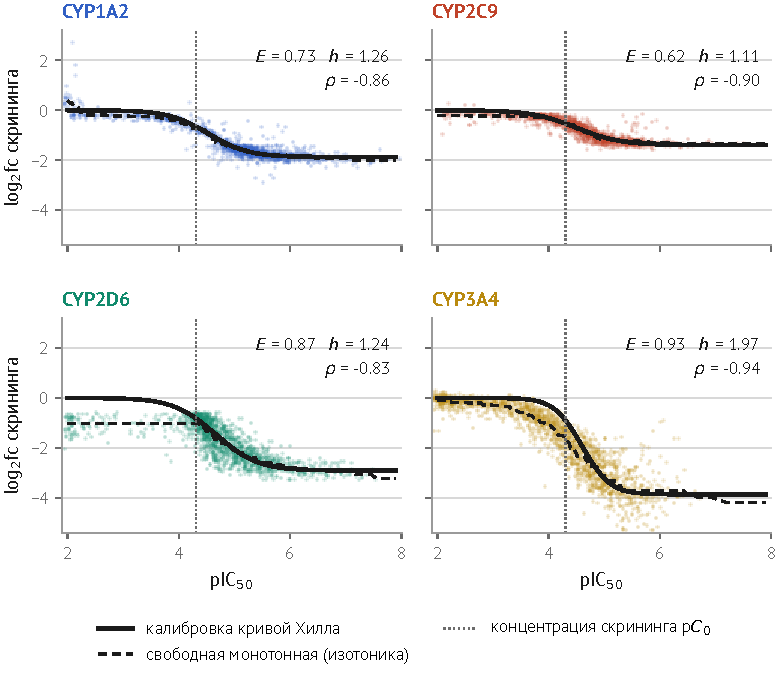
\includegraphics{fig/calib}
\caption{Калибровка. Точки --- соединения, у которых есть и $\pic$, и показание скрининга. Сплошная
линия --- подгонка формой \eqref{eq:hill} с двумя параметрами на фермент, пунктир --- свободная
монотонная кривая, задающая предел для любой монотонной калибровки.}
\label{fig:calib}
\end{figure}

Из этой картинки следует три вещи.

Связь очень сильная: ранговая корреляция от $-0.83$ до $-0.94$. Поэтому скрининг --- почти достаточная статистика. Свободная монотонная калибровка по \emph{измеренному} показанию даёт макро-ST-RAE
0.359 против 0.767 у полной модели по структуре. Знай мы показание скрининга для тестовых соединений,
задача была бы вдвое легче; но на тесте его нет, пересечение теста с первичной библиотекой ровно нулевое.

Хилловская форма теряет немного, но теряет. Стандартное отклонение остатка против свободной монотонной
кривой: 0.231 против 0.208 на 1A2, 0.185 против 0.167 на 2C9, 0.497 против 0.390 на 2D6, 0.612 против
0.499 на 3A4. То есть двухпараметрическая форма жёстче, чем нужно, особенно на 2D6, где свободная кривая
выходит на плато у неактивных, а хилловская тянется к нулю. Это аргумент за монотонную сплайн-поправку
поверх параметрической формы, но не за отказ от неё: форма даёт правильную экстраполяцию там, где данных мало.

Крутизна разная: на 3A4 подобралось $h = 1.97$, на остальных около 1.2. Это свойство постановки
на конкретном ферменте, поэтому калибровка не может быть общей на все четыре.

И этого мало. На CYP3A4 одна пара $(E, h)$ не описывает даже ту популяцию, на которой подогнана:
если расколоть скринированный набор пополам по уровню метки и подогнать каждую половину отдельно,
крутизна выходит 0.503 на нижней и 2.516 на верхней --- пятикратный размах \emph{внутри одного
фермента}, шире всего межферментного разброса. Перенос констант одной половины на другую стоит там
+1.365 против +0.019\ldots+0.067 у остальных трёх. Что за этим стоит --- в разделе~\ref{sec:ident}.

Отдельно проверен планшетный дрейф. Планшетов девять на фермент, и сырой разброс медиан по планшетам
выглядит тревожно: до 0.293 при размахе 0.922. Но планшеты не рандомизированы, активные соединения сидят
кучно, поэтому надо вычесть то, что объясняется составом планшета. После вычитания предсказанного
по $\pic$ разброс падает до 0.039--0.087 при стандартном отклонении остатка 0.19--0.61.

Планшет объясняет от 0.9 до 8 процентов остаточной дисперсии, и разброс по ферментам здесь важнее
диапазона: 3A4 0.9\,\%, 2D6 2.3\,\%, 1A2 3.2\,\%, а 2C9 8.1\,\% --- почти в девять раз больше, чем 3A4.
Вычитание свободной монотонной калибровкой вместо хилловской даёт 0.9, 2.7, 3.8 и 6.7 процента, то есть
та же картина: число --- свойство данных, а не выбора калибровки. Отдельного слагаемого в модели всё же
не требуется, но по другой причине, чем малость доли: даже на 2C9 планшетная компонента даёт
стандартное отклонение около 0.05 в единицах $\log_2$fc, что заметно меньше собственной погрешности
одного показания.

Про обозначение: $E$ в калибровке --- не тот $E$, что в \eqref{eq:theta}. Там предельная
глубина подавления самого соединения, здесь --- параметр установки, вбирающий её динамический диапазон.
Совпадение буквы неудачное и в коде их надо развести.

\subsection{Почему цензурирование получается само}
\label{sec:cens}

Это главный технический аргумент за такую конструкцию. Продифференцируем \eqref{eq:hill} по потенции,
обозначив $x = 10^{h(\pC_0 - \pi)}$:
\begin{equation}
\frac{\partial I}{\partial \pi}
= + E\, h \ln 10 \cdot \frac{x}{(1+x)^2} .
\label{eq:dI}
\end{equation}

Множитель $x/(1+x)^2$ максимален при $x = 1$, то есть ровно когда $\pi = \pC_0$, и равен там одной
четвёртой; при $x \to 0$ и $x \to \infty$ он затухает экспоненциально. Фишеровская информация о $\pi$,
которую несёт одна точка скрининга, пропорциональна квадрату этого множителя.

\begin{figure}[htbp]\centering
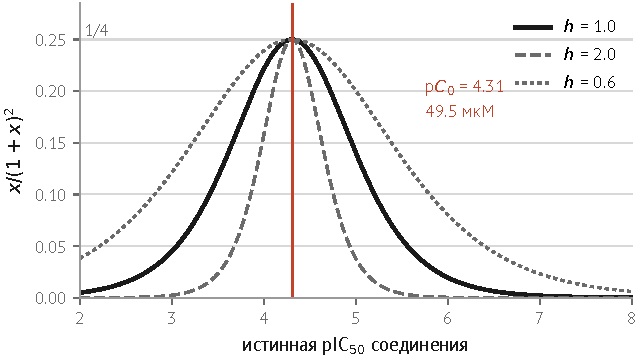
\includegraphics{fig/fisher}
\caption{Сколько информации о потенции несёт одно измерение при концентрации $C_0$. Колокол сосредоточен
вокруг $\pC_0$ с шириной порядка $1/h$ декад и обнуляется в обеих зонах насыщения.}
\label{fig:fisher}
\end{figure}

На практике это значит, что в зонах насыщения градиент по $\pi$ исчезает сам. Для соединения, которое при
49.5 мкМ не подавило ничего, модель извлекает из скрининга мягкое неравенство «активность ниже примерно
такой-то», а не число. Для соединения, подавившего всё, --- неравенство с другой стороны. Никакого
специального кода цензурирования писать не надо, оно следует из формы кривой.

Форма \eqref{eq:dI} видна в данных напрямую: перегиб зависимости показания от $\pic$ на CYP3A4 приходится
на 4.3 (рис.~\ref{fig:calib}), то есть на $\pC_0 = 4.305$ для 49.5 мкМ.

\section{Идентифицируемость}
\label{sec:ident}

Первое, что спросит любой, кто это читает: из одноточечного измерения наблюдается ровно скаляр $I(C_0)$,
а параметров в \eqref{eq:theta} три. Тройка $(\pi, E, h)$ точечно не идентифицируется --- любая кривая,
проходящая через ту же ординату при $C_0$, объясняет данные одинаково хорошо.

Риск конкретный: сеть сбросит остаток в $E$, чтобы подогнать показание скрининга, и испортит $\pi$ ---
единственную величину, которую с неё спрашивают на лидерборде.

Что с этим делаем, по возрастанию силы ограничения.

\subsection{Крутизна --- на уровень фермента}

$h_e$, один скаляр на фермент вместо десятков тысяч. Первую версию делаем вообще с $h_e \equiv 1$.
Оправдание не только техническое: крутизна кривой в такой пробе определяется в основном механизмом
и стехиометрией связывания, а не индивидуальными особенностями лиганда, и подгонка калибровки
(раздел~\ref{sec:calib}) даёт по ферментам устойчивые 1.11--1.97.

\subsection{Глубина: амортизация вместо поштучной подгонки}

Есть два способа получить $E$ для каждого соединения.

\emph{Поштучная подгонка}: у каждого соединения свой свободный параметр $E_m$. Для 4905 соединений
и четырёх ферментов это 19\,620 свободных чисел, каждое подбирается только по данным своего соединения,
и никакой связи между похожими молекулами нет.

\emph{Амортизация}: свободных $E_m$ нет вовсе, есть одна общая функция --- голова сети, получающая
представление молекулы и выдающая ответ:
\begin{equation}
E_{m,e} = \sigma\bigl(u_e^{\top} z_m + c_e\bigr) .
\label{eq:eamort}
\end{equation}

Здесь $z_m$ --- вектор-представление молекулы из общего ствола, $u_e$ и $c_e$ --- веса и сдвиг головы
фермента, сигмоида зажимает ответ в интервал от нуля до единицы. Параметров $4(d+1)$, то есть при $d=256$
чуть больше тысячи, и они обслуживают все соединения сразу, включая те, у которых своей кривой нет.
Отсюда слово: дорогая процедура вывода амортизуется по всем объектам.

Как это работает регуляризатором. Чтобы выдать одному соединению нестандартное
$E$, сети надо сдвинуть его представление, а представление производится общим стволом из структуры, и тот же
ствол обслуживает все похожие молекулы. Подогнать $E$ индивидуально можно только там, где есть структурная
закономерность --- класс молекул, систематически ведущий себя как частичный ингибитор. Если такого класса
нет, а есть только шум подгонки кривой, сети выгоднее выдать всем примерно одинаковое $E$. Формально это
сужение множества гипотез: достижимые наборы $\{E_m\}$ --- уже не произвольный вектор длины $N$, а образ
структурного пространства под гладким отображением. Регуляризация здесь не слагаемое в функции потерь,
а свойство параметризации.

\subsection{А теперь измерения, и они меняют вывод}

Всё сказанное объясняет, почему амортизация безопасна. Но у организаторов опубликованы измеренные $E$:
колонки \texttt{EmaxVsPosCtrl\_direct\_inhibition} с доверительными полосами. Смотреть на них надо было
до всяких рассуждений.

\begin{figure}[htbp]\centering
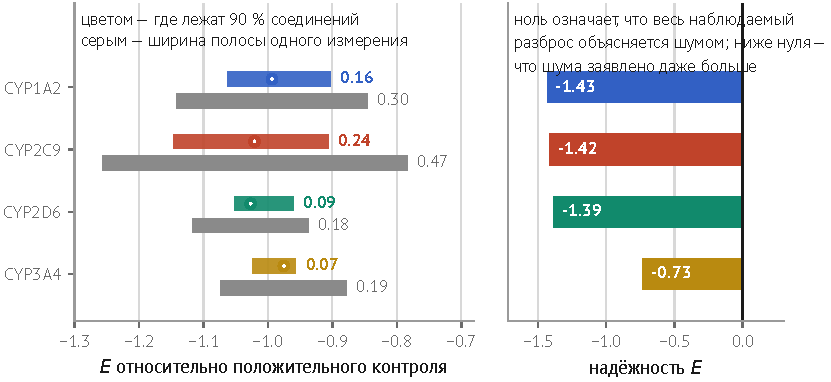
\includegraphics{fig/emax}
\caption{Слева: цветной отрезок --- где лежат 90 процентов соединений, серый --- средняя ширина
доверительной полосы одного измерения. Серый шире цветного на всех четырёх ферментах. Справа: надёжность
по \eqref{eq:rel}, отрицательная везде.}
\label{fig:emax}
\end{figure}

Шкала здесь относительно положительного контроля, поэтому полный ингибитор даёт примерно $-1$.
И вот что оказалось. Весь разброс $E$ \emph{между соединениями} уже, чем заявленная погрешность
\emph{одного} измерения, --- на CYP3A4 втрое, на CYP2D6 вдвое. Иначе говоря, если взять два
случайных соединения, разница их измеренных $E$ в среднем меньше, чем неопределённость каждого
из этих двух чисел по отдельности. Различать соединения по $E$ в такой ситуации нельзя.

Отсюда отрицательная надёжность: от $-0.73$ до $-1.43$. У честной величины она лежит между нулём и единицей;
отрицательная означает, что заявленная дисперсия шума больше всего наблюдаемого разброса. Буквально это
может означать, что полосы посчитаны консервативно, но верхняя оценка сигнала уровня соединения от этого
не меняется --- он не превышает нуля.

Значит амортизация была правильным решением по неправильной причине. Дело не в том, что сеть не
сможет переобучиться на индивидуальные $E$, а в том, что переобучаться там не на чем: сигнала
уровня соединения в этих колонках нет. Вместо головы достаточно одной константы на фермент,
примерно $-1$ у всех четырёх, --- и, если хочется страховки, поштучной поправки с жёстким
штрафом, которую данные обязаны прижать к нулю.

Что наблюдаемая вариация $E$ --- артефакт подгонки кривой, а не химия, видно ещё и по такому
признаку. Связь между измеренным $E$ и активностью почти отсутствует у неактивных и у
активных соединений, но резко усиливается \emph{в средней зоне} --- ровно там, где кривая
доза--эффект обрывается, не дойдя до плато, и подгонщику приходится выбирать глубину
наугад, по гребню. Само по себе это подозрительно. Но решает дело знак: у трёх ферментов
в средней зоне более потентные соединения выглядят давящими \emph{глубже}, а у CYP2D6 ---
наоборот, \emph{мельче}. Химического механизма, который переворачивал бы этот знак от
фермента к ферменту, не существует. Это подпись процедуры подгонки, а не свойство молекул.

Диагностика на будущее остаётся прежней: смотреть разброс выхода головы $E$ отдельно на соединениях
с полной кривой и на соединениях только со скринингом. Если на вторых разброс заметно выше, голова
используется как свалка для остатка.

\section{Механизм пропусков}
\label{sec:mnar}

Полные кривые снимали не для всех: отбор шёл по результату первичного скрининга. Это отбор по зависимой
переменной, то есть missing not at random по построению, и он же --- причина провала на CYP2D6,
измеренная в разделе~\ref{sec:d6}.

Спасает вот что: \emph{переменная отбора наблюдаема}. Скрининг есть для 4375 из 4905 соединений
обучающей выборки, и именно он определял, кого поднимут на подробное измерение.

\subsection{Как раскладывается совместное распределение}

Пишем совместную плотность через скрытую активность $a$, честно:
\begin{equation}
p(y_{\text{крив}}, y_{\text{скр}}, R \mid x,\theta)
= p(R \mid y_{\text{скр}}) \int p(a \mid x,\theta)\, p(y_{\text{скр}} \mid a)\, p(y_{\text{крив}} \mid a)^{R}\, da .
\label{eq:joint}
\end{equation}

Здесь $R$ --- индикатор попадания в подробное измерение, $p(a\mid x,\theta)$ --- что модель думает
об активности до измерений (центр --- предсказание сети, ширина --- признание того, что структура
определяет активность не полностью), два следующих множителя --- шум каждого прибора, зависящий только
от истинной активности. Множитель $p(y_{\text{крив}}\mid a)$ входит в степени $R$, то есть только для
отобранных.

Главный шаг --- вынос $p(R\mid y_{\text{скр}})$ за интеграл. Он законен потому, что решение об отборе
принималось глядя на показание скрининга, а не на скрытую активность: под интегралом по $a$ этот
множитель величины $a$ не содержит.

Применяя цепное правило, получаем рабочую форму:
\begin{equation}
p(y_{\text{крив}}, y_{\text{скр}}, R \mid \theta)
= \underbrace{p(R \mid y_{\text{скр}})}_{\text{без }\theta}
\cdot\; \underbrace{p(y_{\text{крив}} \mid y_{\text{скр}},\, \theta)}_{\text{условно}}
\cdot\; p(y_{\text{скр}} \mid \theta) .
\label{eq:factor}
\end{equation}

Первый множитель не зависит от $\theta$, при дифференцировании логарифма даёт ноль и полностью выпадает
из градиента. Значит можно обучаться на полном правдоподобии, вообще не моделируя процедуру отбора,
и оценки останутся состоятельными. Условие ровно одно: скрининг должен входить в модель как наблюдение.
Если его выбросить, первый множитель перестанет быть отделимым и смещение вернётся. По сути это поправка
хекмановского типа, у которой первая ступень не моделируется, а наблюдается.

Средний множитель обязан быть \emph{условным} по $y_{\text{скр}}$, и это место, где легко ошибиться.
Заменить его на маргинальный $p(y_{\text{крив}}\mid\theta)$ можно только при нулевом собственном латентном
разбросе соединения: два показания меряют одну скрытую активность, они коррелированы, а отбор идёт
по одному из них --- значит среди отобранных распределение второго сдвинуто. Маргинальный множитель
про этот сдвиг не знает.

\subsection{Что даёт симуляция}

Проверено на данных, где истина известна по построению: $a = x^{\top}\beta + \varepsilon$, скрининг у всех,
кривая --- у верхних двадцати восьми процентов по скринингу (порог квантиля 0.72).

\begin{table}[htbp]\centering\small
\begin{tabularx}{\textwidth}{@{}Xrr@{}}
\toprule
Способ подгонки & Смещение, норма & Наклон калибровки \\
\midrule
Только отобранные метки кривых & 0.433 & 0.731 \\
Совместное правдоподобие, отбор по скринингу & 0.019 & 1.012 \\
Только скрининг, все строки (контроль сверху) & 0.002 & 1.000 \\
Отбор по скрытой истине, скрининг у неотобранных не виден & 0.512 & 0.681 \\
\bottomrule
\end{tabularx}
\caption{Сорок повторов, шесть тысяч соединений, в подробное измерение попадает 28 процентов. Наклон
единица означает, что коэффициенты восстановлены без систематического сжатия.}
\label{tab:mnar}
\end{table}

Подгонка по одним отобранным меткам сжимает коэффициенты до 0.73 от истины --- ровно то ограничение
диапазона, которое видно на CYP2D6. Совместное правдоподобие возвращает 1.01.

Четвёртая строка важнее первых трёх. Сломайте условие, то есть сделайте отбор зависящим от скрытой
величины и уберите скрининг у неотобранных, и совместная схема поломается так же, как наивная. Значит
аргумент держится не на общей идее «использовать больше данных», а на наблюдаемости первой ступени
отбора. В наших данных она наблюдаема.

Отдельно измерена цена замены условного множителя на маргинальный. Смещения нет при нулевом латентном
остатке, при $\sigma_{\text{лат}} = 0.35$ оно примерно втрое меньше стандартной ошибки оценки, при
$\sigma_{\text{лат}} = 0.70$ уже сравнимо с ней. И независимо от смещения такая схема занижает собственную
погрешность в 1.18--1.21 раза, потому что считает два коррелированных наблюдения одного соединения
за два независимых свидетельства. Значит голова, предсказывающая $\pic$, должна получать на вход показание скрининга того же соединения.
Или, что то же самое, обе величины должны выводиться из общего латентного слоя с явной ковариацией,
а не из двух независимых голов.

На инференсе скрининга нет, но это не мешает. Условный множитель нужен на обучении, чтобы оценка
не была смещена отбором; на предсказании мы маргинализуем по $y_{\text{скр}}$, что при общем латентном
слое сводится к одному прогону сети.

Оговорка: 530 соединений с кривыми не имеют скрининга, и для них аргумент не работает. По выборке
целиком доля небольшая, но лежит она не равномерно: все 530 --- это метки 3A4, почти четверть всех
кривых этого фермента. Так что на трёх ферментах оговорка пустая, а на 3A4 её надо закрывать --- взвесить
или выкинуть в абляции.

\section{Архитектура}

\subsection{Ствол}

Предобученный химический энкодер $f_\varphi:\ \text{SMILES} \to z \in \mathbb{R}^d$. Организаторы выложили
свои веса (CheMeleon, предобученный D-MPNN, и chemprop-foundation), плюс доступны Minimol и графовые
трансформеры. Ансамблируем по семействам претрейна, а не по сидам одного семейства: ошибки разных
семейств коррелируют слабее, и ансамбль из четырёх разных архитектур даёт больше, чем из восьми запусков
одной. Дообучение через LoRA-адаптеры, чтобы 6.5 тысяч меток кривых не переписали претрейн, обученный
на миллионах молекул.

\subsection{Связь между ферментами: коррегионализация}
\label{sec:icm}

Ферментов четыре, и надо решить, как их связать. Очевидные способы не годятся. Четыре независимые модели:
2C9 не пользуется 2335 метками 3A4, хотя они меряют почти одно и то же. Одна общая голова: 2D6 тянет
в сторону остальных трёх, а он с ними не коррелирует. Общий ствол и четыре независимые головы уже лучше,
но связь между задачами остаётся неявной.

Коррегионализация --- термин из геостатистики: совместное моделирование нескольких величин, измеренных
в одних точках, через общую структуру плюс отдельную матрицу связей между величинами. Простейший вариант,
intrinsic coregionalization model, выносит эту матрицу в явный параметр.

Голова линейная поверх общего представления:
\begin{equation}
\pi_{m,e} = w_e^{\top} g(z_m) + b_e,
\qquad W = [\,w_1\ w_2\ w_3\ w_4\,] \in \mathbb{R}^{d\times 4} .
\label{eq:head}
\end{equation}

Вся связь между ферментами сидит в углах между столбцами $W$: если $w_2$ и $w_4$ смотрят почти в одну
сторону, модели 2C9 и 3A4 читают представление одинаково. Матрица этих углов
\begin{equation}
B = W^{\top}W \in \mathbb{R}^{4\times 4}, \qquad B_{ee'} = w_e^{\top} w_{e'} ,
\end{equation}
и на неё навязывается структура «несколько общих осей плюс своё у каждого»:
\begin{equation}
B \;\approx\; LL^{\top} + \operatorname{diag}(\kappa),
\qquad L \in \mathbb{R}^{4\times r},\quad r = 2 .
\label{eq:icm}
\end{equation}

Строка $e$ матрицы $L$ говорит, насколько фермент участвует в каждой из $r$ общих осей; $LL^{\top}$ ---
общая часть ковариации ранга $r$; $\kappa_e$ --- специфичная часть фермента, то, что есть только у него.
Это обычная факторная модель: $r$ общих механизмов узнавания плюс идиосинкразия.

\begin{figure}[htbp]\centering
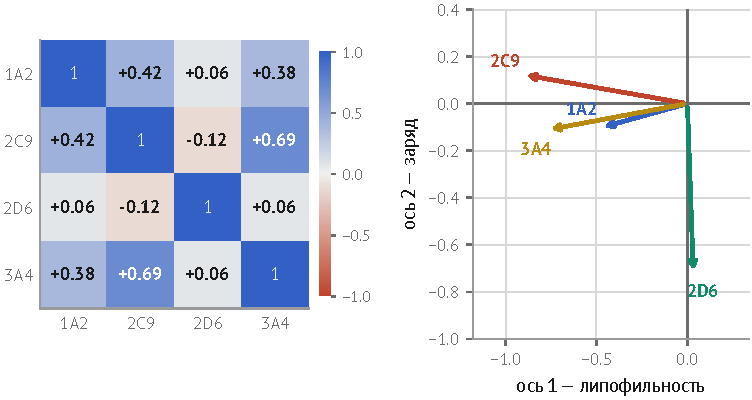
\includegraphics{fig/corr}
\caption{Слева --- ранговая корреляция $\pic$ между ферментами, посчитанная по общим соединениям
(от 230 пар у 2C9--2D6 до 473 у 2C9--3A4). Справа --- нагрузки факторной модели ранга 2 на те же данные:
каждая стрелка показывает, насколько фермент участвует в каждой из двух общих осей. Первая ось нагружает
2C9, 3A4 и слабее 1A2, на 2D6 стоит на нуле; вторая ось --- почти исключительно 2D6.}
\label{fig:corr}
\end{figure}

Данные говорят то же, что раздел~\ref{sec:isoforms}: 2C9 и 3A4 идут в паре ($\rho = 0.688$),
а 2D6 ортогонален всем троим ($0.059$, $-0.120$, $0.056$). Матрица положительно определена, минимальное собственное число 0.287, так что
раскладывать её можно. Нагрузки: ось 1 --- 2C9 $-0.907$, 3A4 $-0.773$, 1A2 $-0.480$, 2D6 $+0.033$;
ось 2 --- 2D6 $-0.726$, остальные около нуля. Специфичные части $\kappa$: 0.759, 0.161, 0.472, 0.390.

Первая ось --- липофильная промискуитетность: крупные жирные молекулы садятся в широкие карманы 2C9 и 3A4.
Вторая --- 2D6 с его солевым мостиком. Общая голова тянула бы 2D6 по первой оси и портила бы его.

Про ранг надо помнить вот что. При четырёх задачах внедиагональ содержит шесть чисел,
а нагрузки ранга 2 дают $4\times 2 = 8$ параметров минус одна степень свободы на вращение, то есть семь.
Модель насыщена: ранг 2 воспроизводит внедиагональ точно не потому, что угадал структуру, а потому что
параметров хватает. По-настоящему ограничивает только ранг 1, и он промахивается максимум на 0.10, причём
весь промах приходится на 2D6. Так что структура ранга 2 --- не сжатие, а способ задать приор и инициализацию. Польза проявится, когда
$B$ будет тянуть головы во время обучения, а не в самой аппроксимации матрицы четыре на четыре.

\paragraph{Регуляризационный член.} Задача --- не дать столбцам $W$ разъехаться в произвольные углы,
когда у фермента мало меток, и притянуть матрицу связей к тому, что видно в данных:
\begin{equation}
\Omega(W) \;=\;
\frac{\lambda_1}{2}\,\bigl\| \rho(W^{\top}W) - \widehat{\rho} \bigr\|_F^2
\;+\;
\frac{\lambda_2}{2}\,\|W\|_F^2 ,
\qquad
\rho(B) = D^{-1/2} B D^{-1/2},\ \ D = \operatorname{diag}(B) .
\label{eq:omega}
\end{equation}

Первое слагаемое: строим $B$, нормируем в корреляционную матрицу, вычитаем эмпирическую $\widehat{\rho}$,
складываем квадраты разностей. Нормировка нужна потому, что притягивать надо \emph{углы}, а не длины
столбцов --- длина отвечает за масштаб предсказания и настраивается данными. Второе --- обычная усадка весов.
Норма Фробениуса $\|A\|_F = \sqrt{\sum_{ij}A_{ij}^2}$ --- евклидова длина матрицы, вытянутой в строку.

Почему именно так, а не поэлементный штраф на $W$. Матрица $W$ определена не однозначно: умножение справа
на любую ортогональную $Q$ не меняет ни $W^{\top}W$, ни предсказания. Регуляризатор обязан обладать той же
симметрией, иначе он штрафует за выбор системы координат, а не за содержание. Обе величины в
\eqref{eq:omega} проходят через $W$ только в виде $W^{\top}W$, поэтому симметрию сохраняют; поэлементный
штраф --- нет.

Низкий ранг входит не штрафом, а параметризацией. Практически проще держать не $W$ со сложным штрафом,
а сразу $L$ и $\kappa$ и строить головы из них:
\begin{equation}
\pi_{m,e} = L_{e\cdot}\, U^{\top} g(z_m) \;+\; \sqrt{\kappa_e}\; s_e^{\top} g(z_m) \;+\; b_e ,
\label{eq:headfac}
\end{equation}
где $U \in \mathbb{R}^{d\times 2}$ --- проекция на общие оси, общая для всех ферментов, а $s_e$ --- вектор
специфичного направления фермента. Тогда $B = LL^{\top} + \operatorname{diag}(\kappa)$ выполняется
по построению, штраф за ранг не нужен, а от \eqref{eq:omega} остаётся притяжение к $\widehat{\rho}$
плюс усадка. Инициализация $L$ и $\kappa$ --- из факторного разложения эмпирической матрицы, причём
именно факторным анализом с итеративной оценкой общностей: наивное собственное разложение полной матрицы
с единицами на диагонали искажает внедиагональные элементы до 0.23, потому что факторы начинают гнаться
за диагональю.

Проверять надо две вещи. Положить $\lambda_1 = 0$ и посмотреть, куда уедет выученная матрица связей
от эмпирической: если далеко, значит либо в представлении есть структура, которой нет в сырых корреляциях,
либо голова переобучается. И сравнить с четырьмя независимыми головами на тех же разбиениях.

\subsection{Механистический блок}

30 признаков, описанных в разделе~\ref{sec:d6}, конкатенируются с $z_m$ либо подаются через FiLM ---
то есть модулируют активации ствола, а не просто дописываются в конец вектора.

Зачем блок нужен, если по метрике он почти ничего не даёт. По ранжированию он избирателен так, как
предсказывает химия, и это подтверждено бутстрапом; модель на одних этих 30 числах воспроизводит большую
часть ранжирующей способности на 2D6 и меньше половины на остальных. Вдобавок он заметно стабилизирует
модель (раздел~\ref{sec:proto}). Считается блок за секунду.

\subsection{Канал артефактов пробы}
\label{sec:artifact}

Как описано в разделе~\ref{sec:bio}, 1A2, 2C9 и 3A4 читаются по флуоресценции, а 2D6 ---
масс-спектрометрией, и собственная флуоресценция соединения или тушение сигнала дают ложное
«ингибирование» только в первых трёх. Это конфаундер, общий для трёх эндпойнтов и отсутствующий
у четвёртого, и он частично объясняет, почему 1A2, 2C9 и 3A4 коррелируют между собой.

Добавляем скалярный признак-помеху (протяжённость сопряжения, известные хромофорные каркасы) с обучаемым
коэффициентом, входящий только в три флуоресцентных эндпойнта. Это поправка на конфаундер с известной структурой, а не ещё один признак в общую кучу: модель получает
возможность объяснить часть общей вариации артефактом, а не химией.

\subsection{Головы}

\begin{itemize}
\item $\pi$-голова --- линейная поверх \eqref{eq:headfac}, выход в $\mathbb{R}$.
\item $(\sigma^-, \sigma^+)$-головы --- гетероскедастичные, через softplus; обучаются через
\eqref{eq:split}. Границы интервалов лежат в данных и обычно никем не используются, а решающему слою
они нужны.
\item $E$ --- константа на фермент, по итогам раздела~\ref{sec:ident}, плюс опциональная штрафуемая поправка.
\item $\Delta$-голова --- softplus, отдельная. Не разность двух независимых регрессий: шум двух плеч
коррелирован и частично сокращается в разности, поэтому предсказывать сдвиг напрямую точнее. Измерено:
0.255 против 0.323 по MCC на 3A4 в пользу отдельной головы.
\end{itemize}

\section{Функция потерь и обучение}

\begin{equation}
\mathcal{L} = \sum_{m,e}
\Bigl[\lambda_{\text{крив}}\ell_{\text{крив}} + \lambda_{\text{tdi}}\ell_{\text{tdi}}
+ \lambda_{\max}\ell_{\max} + \lambda_{\text{скр}}\ell_{\text{скр}}\Bigr]
+ \lambda_{\text{полоса}}\ell_{\text{полоса}} + \lambda_{\text{st}}\ell_{\text{st}} + \Omega(W) .
\label{eq:loss}
\end{equation}

Первые четыре слагаемых --- правдоподобия четырёх источников из раздела~\ref{sec:gen}. Пятое обучает головы полос
$(\sigma^-,\sigma^+)$. Шестое --- клипованная L1 из \eqref{eq:strae}, посчитанная на обучающих полосах;
она выравнивает функцию потерь с метрикой соревнования, потому что правдоподобие оптимизирует не совсем то,
по чему считается лидерборд. Последнее --- регуляризатор \eqref{eq:omega}.

\subsection{Батчинг по молекулам, а не по строкам}

Единица батча --- молекула со всеми её наблюдениями по всем источникам и ферментам. Иначе теряется смысл конструкции: латентная $\theta_{m,e}$ общая для кривой, Emax и скрининга,
и градиенты от них должны сходиться на одном узле в пределах одного шага. Батч по строкам превращает конструкцию обратно
в обычную многозадачную модель с общим стволом.

\subsection{Двухэтапная калибровка}

Если учить $\psi_e = (s_e, b_e, \sigma_e)$ совместно с сетью с самого начала, есть вырожденное решение:
сеть подстраивает $\pi$ под удобную калибровку вместо обратного. Порядок такой.

\begin{enumerate}
\item На подмножестве, где есть и кривая, и скрининг, фиксируем $\pi$ равным опубликованному и подгоняем
12 скаляров $\psi$ напрямую. Задача низкоразмерная, решается за секунды; результат --- в
разделе~\ref{sec:calib}.
\item Обучаем сеть с замороженной $\psi$.
\item Размораживаем $\psi$ с маленьким шагом обучения на последних эпохах.
\end{enumerate}

\subsection{Веса источников}

Стартуем с $\lambda \propto 1/n_{\text{источника}}$, чтобы 17.5 тысяч точек скрининга не задавили
6.5 тысяч меток кривых. Потом пробуем гомоскедастичное взвешивание по неопределённости: каждому источнику
свой обучаемый $\log \sigma^2$, веса выводятся из него, и модель сама решает, какому источнику доверять.
Проверяем это абляцией, а не берём на веру: приём известен, но на маленьких выборках его собственный шум
иногда съедает пользу.

\section{Неопределённость}
\label{sec:unc}

\emph{Статус раздела.} Как и предыдущий, это замысел, а не работающий код: раздел написан до
измерений и с тех пор правился один раз. Ни одно число документа на описанной здесь
конструкции не получено.

На выходе нужно распределение, а не число, и не ради красоты: решающий слой
(раздел~\ref{sec:decision}) без него не работает вообще --- ему нужно знать не только, какую
активность модель считает наиболее вероятной, но и насколько она в этом уверена.

Неопределённость принято делить надвое, и деление это не педантизм, а рабочий инструмент.
\emph{Эпистемическая} часть --- та, что происходит от нашего незнания: похожих молекул в
обучении было мало, и модель просто не знает, что тут бывает. Она уменьшается, если добавить
данных. \emph{Алеаторная} часть --- собственный шум измерения: сколько ни добавляй молекул,
прибор точнее не станет. Различать их нужно потому, что реагировать на них надо
по-разному, и потому что трансдуктивный слой опирается ровно на первую.

Собирается распределение из трёх частей.

\emph{Ансамбль} по сидам и семействам энкодеров даёт эпистемическую часть --- ту неопределённость, которая
происходит от незнания правильной модели и падает с ростом данных. Дешёвые альтернативы, если бюджет
не позволяет держать ансамбль: SWAG или лапласовское приближение на последнем слое.

\emph{Гетероскедастичные головы} $(\sigma^-,\sigma^+)$ дают алеаторную часть --- шум прибора, который
не уменьшить никаким количеством данных.

\emph{Конформная калибровка} на разбиении, воспроизводящем дизайн теста. Обычная конформная калибровка
даёт маргинальное покрытие: в среднем по всей выборке 90 процентов заявленных интервалов накрывают истину.
Нам нужно условное: у неактивных соединений полосы широкие по построению, и если модель систематически
промахивается на активных, среднее покрытие это замаскирует. Проверяем покрытие по зонам активности
отдельно, при необходимости берём мондриановский вариант с зонами в качестве таксономии.

Разделять алеаторную и эпистемическую части нужно не для отчёта, а для трансдуктивного слоя:
эпистемическая компонента велика там, где мало похожих обучающих примеров, а тест как раз состоит
из серий аналогов вокруг известных хитов.

\section{Решающий слой}
\label{sec:decision}

Предсказательное распределение получено. Осталось превратить его в то, что просят отправить: одно число
для регрессии и один бит для классификации. Это отдельный шаг, и правильный ответ зависит от метрики.

\subsection{Регрессия: вывод}

Пусть $(L, H)$ --- случайные границы доверительного интервала будущего измерения. Риск точечной оценки
по \eqref{eq:strae}:
\begin{equation}
R(\hat y) = \E\bigl[(\hat y - H)_+\bigr] + \E\bigl[(L - \hat y)_+\bigr],
\qquad
R'(\hat y) = F_H(\hat y) - \bigl(1 - F_L(\hat y)\bigr) .
\label{eq:risk}
\end{equation}

Здесь $F_L$ и $F_H$ --- функции распределения нижней и верхней границ. Производная считается просто:
сдвигая $\hat y$ вправо на $d\hat y$, мы добавляем штраф там, где $H$ уже левее (вероятность $F_H(\hat y)$),
и снимаем штраф там, где $L$ ещё правее (вероятность $1 - F_L(\hat y)$).

Оба слагаемых в \eqref{eq:risk} выпуклы, значит стационарная точка глобальна, и условие оптимума
\begin{equation}
F_L(\hat y^*) + F_H(\hat y^*) = 1 .
\label{eq:opt}
\end{equation}

Это условие $F_M(\hat y^*) = 1/2$ для равновесной смеси $M = \tfrac12 L + \tfrac12 H$. Рецепт
получается такой: взять $S$ сэмплов из предсказательного распределения, для каждого посчитать пару
$(l, h)$, свалить все $2S$ чисел в один массив и взять медиану. В вырожденном случае $L = H = Y$ условие
даёт апостериорную медиану, а не среднее --- что и следовало ожидать от метрики на основе L1.

Вывод верный, проверен численно. А вот прежнее утверждение о том, что для неактивных соединений оптимум
смещается вверх, оказалось неверным. Оно опиралось на предположение, что полосы у неактивных сильно
асимметричны вниз. Измерение показало, что полосы почти симметричны везде: медиана асимметрии $b-a$
(где $a = y - l$, $b = h - y$) не превышает 0.13 логарифмической единицы ни в одной ячейке, причём
у трёх ферментов из четырёх у неактивных знак отрицательный.

\begin{table}[htbp]\centering\small
\begin{tabularx}{0.88\textwidth}{@{}Xrrrrr@{}}
\toprule
Вариант решающего слоя & 1A2 & 2C9 & 2D6 & 3A4 & Макро \\
\midrule
Сырое предсказание модели & 0.879 & 0.691 & 0.980 & 0.519 & 0.767 \\
Пул границ, полосы предсказаны моделью & 0.889 & 0.710 & 1.002 & 0.540 & 0.785 \\
Пул границ с истинными полосами (оракул) & 0.864 & 0.670 & 0.971 & 0.505 & 0.752 \\
\bottomrule
\end{tabularx}
\caption{Один и тот же предиктор, разные решающие слои, те же фолды. Оракул недостижим --- он знает
истинные границы, --- и задаёт потолок всей затеи.}
\label{tab:decision}
\end{table}

Потолок решающего слоя под ST-RAE --- 0.015 макро, около двух процентов относительно, и это при оракульном
знании полос. Реалистичная версия с предсказанными полосами сейчас теряет 0.018. Причина видна из второго следствия раздела~\ref{sec:task}: метрику определяют активные соединения, а у них полосы
узкие ($a \approx b \approx 0.1$) и симметричные, эксплуатировать нечего. Широкие полосы у неактивных,
но они почти не дают вклада.

Слой понижается в приоритете: делать после того, как заработает всё остальное, и только если
гетероскедастичные головы дадут заметно лучшую оценку полос, чем нынешний бустинг.

\subsection{TDI: здесь слой окупается}

Метка TDI не измеряется напрямую. Она вычисляется из двух измеренных $\pic$ --- прямого плеча
и плеча с преинкубацией (раздел~\ref{sec:tdi}) --- по составному правилу, и правило воспроизводит
опубликованные метки без единого исключения: 2334 из 2334 для 3A4 и 1493 из 1493 для 2D6. Проверено и покомпонентно: убрать любое
из двух слагаемых, и правило начинает пропускать положительные (84 пропуска на 3A4 и 51 на 2D6 без
второго), а взять любое слагаемое по отдельности --- сотни ложных срабатываний.

Значит вероятность «да» надо считать интегрированием правила по совместному предсказательному
распределению, а не отдельной сигмоидой:
\begin{equation}
p_i = \Pr\bigl(\pi > 4,\; \Delta > \log_{10} 2\bigr)
    + \Pr\bigl(\pi \le 4,\; \pi + \Delta > 4 + \log_{10} 2\bigr) .
\label{eq:tdirule}
\end{equation}

Два слагаемых --- два случая правила разметки, разобранных в разделе~\ref{sec:tdi}. Считать это надо
совместно: $\pi$ и $\Delta$ коррелированы, перемножать вероятности по отдельности нельзя. На практике ---
Монте-Карло по сэмплам из ансамбля.

Дальше порог. Как отмечено в разделе~\ref{sec:task}, MCC не раскладывается по объектам, поэтому 0.5 почти всегда
неоптимален. При калиброванных $p_i$ берём порог, максимизирующий ожидаемый MCC на всём наборе из 750.
Два способа, оба дешёвые: подстановка ожидаемых счётчиков $\E[TP] = \sum_{i:\,p_i > t} p_i$ со свипом
по $t$, либо Монте-Карло по пуассон-биномиальному распределению меток.

\begin{figure}[htbp]\centering
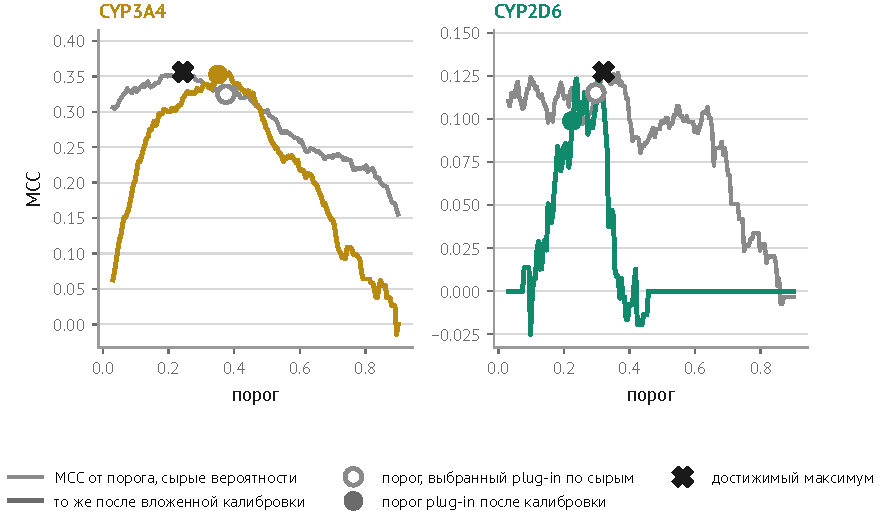
\includegraphics{fig/mcc}
\caption{MCC как функция порога. Слова «при калиброванных $p_i$» оказались не формальностью:
на сырых вероятностях подстановочный порог промахивается мимо максимума. На CYP3A4 он даёт 0.325 при
достижимых 0.356, на CYP2D6 --- 0.115 при 0.127. На 3A4 промах стоит больше половины всего выигрыша
от подбора порога.}
\label{fig:mcc}
\end{figure}

На сохранённых вероятностях бустинга средняя предсказанная вероятность равна 0.256 против настоящей доли
положительных 0.326 на 3A4 и 0.079 против 0.217 на 2D6. Подстановочный метод берёт на 3A4 порог 0.375
и даёт MCC 0.325, тогда как оптимум при 0.258 даёт 0.358 --- потеря 0.033. Вложенная калибровка Платта
возвращает почти всё: потеря падает до 0.003, показатель Брайера с 0.2075 до 0.1853, чистый выигрыш
$+0.028$ MCC. Больше, чем даёт любая перестановка признаков в наших абляциях.

На 2D6 не окупается. Калибровка чинит калибровку (средняя предсказанная с 0.079 до 0.217, Брайер
с 0.199 до 0.169), а MCC не растёт: изотоническая сжимает достижимый максимум с 0.127 до 0.108, Платт
уводит порог не туда. При MCC порядка 0.12 и 260 положительных на обучение калибратора его собственный
шум съедает пользу.

В архитектуру идёт связка «вложенная калибровка, затем подстановочный порог», с абляцией на каждом
эндпойнте отдельно.

Незакрытая дыра: вероятностная версия \eqref{eq:tdirule} с интегрированием по ансамблю не запускалась
ни разу. Все измеренные варианты правила --- детерминированные подстановочные.

\section{Трансдуктивный слой}
\label{sec:trans}

Про тест известно больше, чем обычно, и этим можно пользоваться. Аккуратно.

\emph{Статус раздела.} Обе описанные конструкции с тех пор упёрлись в измерение, и по-разному:
перекалибровка под тестовую маргиналь остаётся \emph{открытым решением}, которое нельзя проверить
изнутри, а серийный случайный эффект \emph{закрыт} --- ниже сказано, чем именно. Зато появилась одна
величина, которую можно посчитать \emph{на самом тесте} без единой метки, и она в конце раздела.

\subsection{Сдвиг распределения}

Тест обогащён активными по трём ферментам и близок к фону по четвёртому (раздел~\ref{sec:data}). Это ковариатный сдвиг
с индуцированным сдвигом меток: $p_{\text{тест}}(y) \ne p_{\text{обуч}}(y)$. Модель, откалиброванная
на обучающей маргинали, будет систематически занижать активность тестовых соединений. Лечится
перекалибровкой под ожидаемую тестовую маргиналь, оценённую из известной конструкции набора, и проверяется
на разбиении, воспроизводящем дизайн теста.

\subsection{Серийный случайный эффект}

Тест --- серии аналогов вокруг якорей, но охват этой структуры зависит от того, что считать серией:
при рабочем пороге 0.35 в группы по пять и более членов попадает 155 соединений из 750, при 0.48 ---
496 (раздел~\ref{sec:data}). Естественно предположить, что соединения одной серии имеют общий сдвиг:
\begin{equation}
\hat y_i = f(x_i) + b_{s(i)},
\qquad b_s \sim \mathcal{N}\bigl(\mu(\text{якорь}_s),\, \tau^2\bigr) .
\label{eq:series}
\end{equation}

Здесь $s(i)$ --- серия, к которой относится соединение $i$, $b_s$ --- её общий сдвиг, $\mu(\text{якорь}_s)$ ---
центр приора, привязанный к активности якоря, $\tau$ --- насколько сильно мы разрешаем серии отклоняться
от него.

Соблазн стянуть предсказание к активности якоря надо давить. Медианная разница $\pic$ в обучающих парах
со сходством Танимото 0.6--0.85 составляет от 0.33 до 0.68 логарифмической единицы. Обрывы активности
реальны: похожие молекулы регулярно различаются в разы. Значит $\tau$ должно быть порядка 0.5, а не 0.1,
и оценивать его надо по обучающим парам при том же уровне сходства, а не подбирать.

Оговорка, которая тут важнее самого числа: пар в этой полосе всего 601 на всю обучающую выборку, и обе
метки есть лишь у 30 из них на 1A2, 15 на 2C9, 23 на 2D6 и 510 на 3A4. То есть три из четырёх медиан
стоят на полутора-трёх десятках пар, и приводить их с двумя знаками --- преувеличение точности. Вывод
про порядок $\tau$ от этого не страдает: он одинаков при любом прочтении этих чисел. А вот оценивать
$\tau$ по обучающим парам пофермент, как здесь предлагается, на 2C9 не выйдет --- пятнадцати пар для
этого мало, и придётся либо пулить ферменты, либо расширять полосу сходства.

Проверять эффект от \eqref{eq:series} можно только на псевдотестовых сериях: на случайном разбиении
он покажет ложный выигрыш, потому что там соседи по серии лежат в обучении.

\emph{Слой закрыт, и закрыт дважды.} Первое: направление проверяется без единой тестовой метки ---
достаточно сравнить, насколько модель разводит членов серии, с тем, насколько их разводит химия.
Модель разводит \emph{слабее} в полтора-три раза на каждом ферменте, то есть она уже переглажена
внутри серии, и стягивание к якорю только усугубило бы ошибку.

Обратное лечение --- \emph{растянуть} внутрисерийные отклонения --- напрашивается и тоже не проходит,
но по другой причине, и она тоньше. Растяжение монотонно внутри группы, поэтому внутрисерийный порядок
не меняет вовсе; вся его польза межсерийная и существует ровно тогда, когда внутрисерийные отклонения
модели \emph{информативны}, а не просто сжаты. Отношение масштабов этого не различает: чистый шум дал
бы ту же картинку. Различает коэффициент затухания --- корреляция отклонений, умноженная на отношение
размахов, --- и на CYP3A4, единственном ферменте, где серий хватает для оценки, он равен 0.833. Ниже
единицы: отклонения зашумлены сильнее, чем сжаты, и растяжение усилило бы шум.

Второе, и это ограничение на весь раздел: \emph{наша кросс-валидация к серийной оси структурно слепа}.
При сходстве 0.60 в сериях лежит 10.2 процента обучающих молекул против 69.1 процента тестовых ---
всемеро. Любая оценка серийного эффекта, снятая на нашей выборке, ограничивает не тест, а популяцию, в
которой серий почти нет.

\subsection{Что о тесте всё же можно узнать без меток}

Одна величина считается прямо на 750 закрытых молекулах и меток не требует: доля пар, о порядке которых
члены ансамбля \emph{расходятся}. Спорна пара или нет --- вопрос о том, одинаково ли её упорядочили
пять моделей, а не о том, кто прав.

Вне фолда таких пар 27.4 процента, на тесте 27.9 --- отношение 1.012. Подача, стало быть, ровно
настолько же внутренне согласована на тесте, насколько была на кросс-валидации, и точность на спорных
парах переносится как измерена. Это отрицательный результат про опасение, а не выигрыш; но после того
как выяснилось, что к аналоговой структуре теста наша проверка слепа, утверждение о тесте, не
требующее меток, стоит здесь дороже обычного.

\section{Протокол оценки}
\label{sec:proto}

Что считать выигрышем, решается до эксперимента. Иначе за два месяца можно уехать сколь угодно далеко.

\subsection{Три уровня строгости разбиения}

\emph{Случайное пятикратное} --- верхняя граница, полезна только для отладки. Оптимистичнее кластерного
примерно вдвое по $R^2$.

\emph{Кластерное по Бутине при пороге 0.35} --- рабочий режим, все числа этого документа получены на нём.
Соединения группируются по сходству, и целый кластер целиком уходит в отложенный фолд, так что модель
не может узнать соединение по его близкому родственнику в обучении.

\emph{Разбиение под дизайн теста} --- ближе всего к реальности. Псевдотестовый фолд строится тем же
алгоритмом, что и настоящий тест: берём хит из обучающей выборки, забираем его 10 ближайших соседей,
держим всю серию снаружи.

\subsection{Насколько наша проверка похожа на тест}

Прежде чем отбирать модели, надо спросить: наша кросс-валидация вообще такой же трудности, как тест?
Мера простая --- сходство соединения с ближайшим к нему обучающим.

\begin{figure}[htbp]\centering
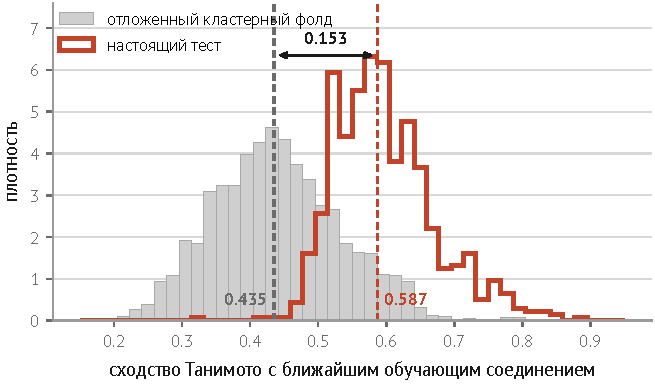
\includegraphics{fig/nnsim}
\caption{Насколько далеко проверяемое соединение от того, что модель видела. Разрыв медиан 0.153,
и он идёт в неожиданную сторону: наша проверка труднее теста.}
\label{fig:nnsim}
\end{figure}

У отложенного кластерного фолда медиана 0.435 и доля соединений со сходством выше 0.7 равна половине
процента. У настоящего теста медиана 0.587, и таких соединений каждое десятое.

Приятная половина: 0.767 --- оценка снизу, на лидерборде должно быть лучше. Неприятная: мы отбираем
модели по способности экстраполировать на чужую химию, а тест награждает за интерполяцию внутри серии
аналогов. Это разные умения, и лучшая по нашей сетке модель не обязана быть лучшей там. Эту дыру
закрывает разбиение под дизайн теста, и теперь у него есть цена, выраженная числом.

\subsection{Устойчивость к разбиению}

Все числа регрессионного трека изначально стояли на одном разбиении --- кластеры Бутины, раскиданные
по фолдам генератором с зерном ноль. Парный бутстрап покрывал случайность выборки соединений, но не
случайность самого разбиения. Прогон на других зёрнах меняет только то, как кластеры распределяются
по пяти фолдам; кластеризация, признаки, гиперпараметры и код те же.

\begin{figure}[htbp]\centering
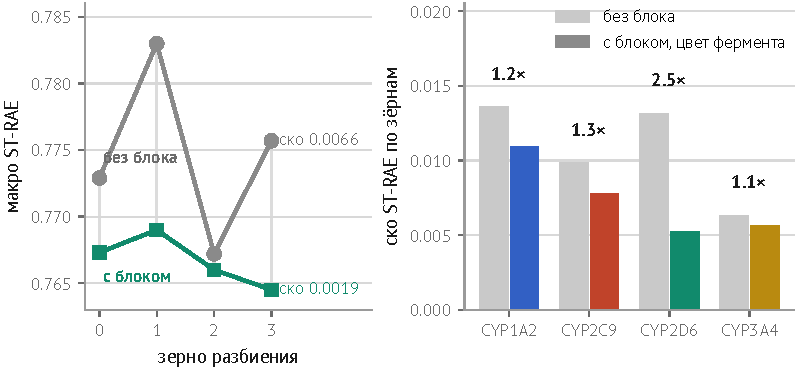
\includegraphics{fig/seeds}
\caption{Слева --- макро-ST-RAE на четырёх зёрнах разбиения. Справа --- стандартное отклонение по этим
четырём зёрнам, по ферментам. Механистический блок снижает зависимость от разбиения в 3.4 раза
по макро, и падение сосредоточено на 2D6.}
\label{fig:seeds}
\end{figure}

Абсолютный уровень плавает: 0.7729, 0.7830, 0.7672, 0.7757 для набора без механистического блока.
Стандартное отклонение 0.0066, размах 0.0158 --- больше, чем весь эффект, ради измерения которого
строилась абляционная сетка. Любое число вида «макро 0.767» без указания разбиения имеет точность
до первого знака после запятой, не до третьего.

Направление держится: разность отрицательна на всех четырёх зёрнах ($-0.0056$, $-0.0140$, $-0.0012$,
$-0.0112$), Спирмен растёт тоже на всех четырёх, а на 2D6 от $+0.033$ до $+0.052$. Бутстрап на одном
разбиении накрывал ноль; четыре разбиения показывают, что знак устойчив, хотя величина гуляет в десять раз.

Самое интересное здесь в разбросах, а не в средних. Набор без блока имеет по зёрнам разброс 0.0066,
с блоком --- 0.0019, в 3.4 раза меньше. По ферментам эффект сосредоточен там, где и должен: на 2D6
разброс падает с 0.0132 до 0.0052, а на 3A4 почти не меняется.

Похоже, двадцать восемь механистических чисел дают модели опору, не зависящую от того, какие аналоги
попали в обучающие фолды. Фингерпринт такой опоры не даёт: он узнаёт соединение по соседям, и когда
соседи уезжают в отложенный фолд, узнавание рассыпается. Главная польза блока, видимо, в этом,
а не в приросте среднего.

Протокол из-за этого меняется. Любое сравнение вариантов идёт на фиксированном наборе из нескольких
разбиений и отчитывается разностью на каждом плюс разбросом. Одно разбиение годится для отладки
и не годится для решения, что отправлять.

\subsection{Парный бутстрап}

Любое сравнение двух вариантов --- только на одном и том же разбиении и с парным бутстрапом
по соединениям: 2000--3000 пересборок, для каждой обе метрики пересчитываются на одной и той же
пересобранной выборке, докладывается распределение разности и доля пересборок, где стало хуже.
Разность без интервала не является результатом.

Для макро надо ресэмплить соединения общей таблицы, а потом для каждого фермента брать те из них,
у кого есть метка --- так сохраняется корреляция между ферментами. Считать четыре независимых бутстрапа
и усреднять нельзя.

\subsection{Сетка абляций}

Каждая строка снимается с парным бутстрапом относительно предыдущей, на нескольких зёрнах.

\begin{enumerate}
\item Фингерпринт и дескрипторы, бустинг. Базовая линия.
\item Предобученный энкодер вместо ручных признаков, одна голова на эндпойнт.
\item Плюс коррегионализация \eqref{eq:icm}.
\item Плюс механистический блок и канал артефактов пробы.
\item Плюс скрининг через \eqref{eq:scr}: главная проверка всей идеи.
\item Плюс Emax и плечо с преинкубацией в общее правдоподобие.
\item Плюс ансамбль и конформная калибровка.
\item Плюс решающий слой: отдельно для регрессии, отдельно для MCC.
\item Плюс трансдуктивный слой.
\end{enumerate}

Строка 5 --- точка, на которой конструкция оправдывается или не оправдывается. Обязательный контроль
к ней: сильная многозадачная базовая линия на тех же признаках и том же энкодере, обученная на одних
метках кривых. Если совместное правдоподобие её не обыгрывает, это отрицательный результат, и он идёт
в отчёт как есть.

\section{Что уже измерено и не работает}

Это тоже результат, и он объясняет, почему решение выглядит так, а не проще. Если скрининг настолько
информативен, зачем городить совместное правдоподобие? Нельзя ли подключить его в лоб? Проверены
три способа.

\begin{table}[htbp]\centering\small
\begin{tabularx}{\textwidth}{@{}Xrrrl@{}}
\toprule
Подход & ST-RAE & $\Delta$ к своей базе & $\rho$ & $\Delta\rho$ \\
\midrule
Скрининг как признак, в лоб & 0.921 & $+0.138$ & 0.566 & $+0.009$ \\
То же с честной вложенной схемой & 0.788 & $0.000$ & 0.559 & $+0.006$ \\
Два этапа: скрининг, затем пересчёт & 1.006 & $+0.212$ & 0.561 & $+0.010$ \\
Смесь двух маршрутов пополам & 0.803 & $+0.009$ & 0.587 & $+0.036$ \\
\bottomrule
\end{tabularx}
\caption{Разности считаются от базовой линии \emph{того же прогона}: 0.783, 0.788, 0.794, 0.794.
Расходятся они не случайно --- это три разных скрипта с тремя разными конфигурациями, см. ниже, ---
поэтому сравнивать строки между собой по абсолютной величине нельзя, только по разностям.}
\label{tab:neg}
\end{table}

\emph{Почему базовые линии не совпадают.} Три скрипта, давшие эту таблицу, строят разбиение по
фингерпринту в 1024 бита, тогда как абляционная сетка и все остальные числа документа --- по 2048.
При 1024 битах кластеризация даёт 4694 кластера против 4703, и вектор фолдов другой: дайджест
\texttt{d7b7ca15} против \texttt{2d93c198}. Поэтому ни одно число этой таблицы не сопоставимо
с 0.767 из раздела~\ref{sec:proto}: различаются не только модели, но и выборки, на которых
они отложены.

Между собой фолды у трёх скриптов совпадают, и расхождение базовых линий объясняется целиком
конфигурацией: шесть физико-химических признаков против восьми даёт 0.783 против 0.788, а
250 итераций бустинга против 200 --- 0.788 против 0.794. Оба различия детерминированы и
воспроизводятся при повторном запуске точно. Разброс в 0.011 --- это не шум прогона, а три
разные модели на общих фолдах.

\emph{Скрининг как признак, в лоб.} Обучаем вспомогательную модель предсказывать $\log_2$fc, её выход
подаём как признак в основную. Ошибка --- вспомогательный признак посчитан моделью, для которой
обучающие строки основной модели были внутренними. На них он точнее, чем окажется на отложенных,
основная модель учится на него опираться, и опора рассыпается там, где её проверяют: 0.783 против
0.921. На честной вложенной схеме выигрыш ровно нулевой. Разница между 0.783 и 0.921 целиком
артефакт процедуры.

\emph{Двухэтапная инверсия.} Предсказать $\log_2$fc, потом перевести в $\pic$ монотонной калибровкой.
Обязана выдать число там, где правдоподобие плоское: в зонах насыщения из раздела~\ref{sec:cens} калибровка
не определена, и любое значение оттуда одинаково согласуется с показанием. Результат: абсолютная шкала
разваливается, а ранговая информация в среднем сохраняется --- но только в среднем, см. ниже.

\emph{Смесь.} Полусумма двух маршрутов. Стоит $+0.009$ ST-RAE и покупает $+0.036$ Спирмена, причём ранг
растёт на всех четырёх ферментах. Это уже почти приемлемый обмен, но он не решает задачу, а балансирует
между двумя плохими решениями.

Общий вывод: информация в скрининге есть, но «ранг улучшается всегда» --- верно только для макро. Поферментно двухэтапная инверсия ранг роняет, причём на том ферменте, вокруг которого построен весь документ: на 2D6 Спирмен идёт с 0.398 до 0.362, на 3A4 с 0.749 до 0.747, и держится макро только за счёт 1A2 ($+0.048$) и 2C9 ($+0.028$). Смесь двух маршрутов --- единственный из трёх вариантов,
который поднимает ранг на всех четырёх.

Информация в скрининге, таким образом, есть, и вся проблема в том, как перевести её в абсолютную шкалу
$\pic$, не потеряв ранг там, где он нам нужнее всего. Этим занимается совместное правдоподобие через
общую латентную кривую.

Сюда же два отрицательных результата из предыдущих разделов: решающий слой под ST-RAE имеет потолок
0.015 макро и в реалистичной версии сейчас теряет 0.018; выигрыш механистического блока по ST-RAE
неотличим от нуля и поштучно, и на макро.

\section{Что сломается и по какому признаку это видно}

\begin{table}[htbp]\centering\small
\begin{tabularx}{\textwidth}{@{}p{40mm}Xp{42mm}@{}}
\toprule
Режим отказа & Признак & Реакция \\
\midrule
Совместное правдоподобие не обыгрывает многозадачную базовую линию
& строка 5 абляции внутри интервала парного бутстрапа на нескольких сидах
& зафиксировать как отрицательный результат, отправлять многозадачную модель; решающий и трансдуктивный слои от неё не зависят \\
Голова $E$ как свалка для остатка
& разброс выхода $E$ на соединениях только со скринингом заметно выше, чем на соединениях с кривой
& заменить на константу на фермент, зафиксировать $h_e = 1$ \\
Калибровка зависит от соединения, а не только от фермента
& остатки \eqref{eq:scr} систематически изогнуты по $\pi$ на подмножестве с полными кривыми
& монотонная сплайн-поправка поверх хилловской формы либо смесь двух режимов \\
Серийный приор переобучается на якоря
& на псевдотестовой \emph{страте} (328 соединений, из них 267 с меткой 3A4;
раздел~\ref{sec:proto}) модель с \eqref{eq:series} хуже, чем без. На остальных трёх
ферментах страта слишком мала, и триггер там не срабатывает вовсе
& увеличить $\tau$ или снять слой \\
Конформные интервалы калиброваны маргинально, но не условно
& покрытие по зонам активности расходится с номинальным
& мондриановский конформал с зонами как таксономией \\
Расхождение локальной оценки с промежуточной таблицей
& макро отличается больше чем на 0.03 --- столько даёт переход к тестовой геометрии
на нашей же выборке (0.767 против 0.739 на верхней четверти по сходству)
& чинить разделы \ref{sec:proto} и трансдуктивный слой, а не архитектуру \\
\bottomrule
\end{tabularx}
\caption{Каждому риску --- наблюдаемый признак и заранее решённая реакция.}
\end{table}

Планшетный дрейф был в этом списке и снят измерением (раздел~\ref{sec:calib}).

\section{Что не проверено}

Список на момент выпуска документа.

\emph{Совместная модель запущена в минимальной форме, полная --- нет.} Строка 5 абляции больше
не пуста: общий ствол с двумя головами и переключателем при слагаемом скрининга измерен на четырёх
сидах, результат в разделе~\ref{sec:neg}. Коротко: канал несёт извлекаемую информацию, но
получить её в единицах метрики удаётся только вместе с перекалибровкой после модели, а
поферментно эффект меняет знак и на 2D6 отрицателен.

Незакрытым остаётся следующее. Измерены две свободные головы над общим стволом, то есть
многозадачность; конструкция раздела~\ref{sec:gen}, где скрининг ограничивает $\pi$ через
фиксированную калибровку, --- отдельный объект, и он тоже измерен: результат в
разделе~\ref{sec:neg}, и он хуже, а не лучше.

\emph{Механизм порчи одноголовой руки не установлен, и объясняющая переменная не
идентифицирована.} Шумовая лестница запущена и описана в разделе~\ref{sec:neg}. Она дала
внутрифермент\-ную причинность, которой не было, и сняла информационное объяснение: при почти
мёртвом канале потеря не падает, а растёт. Но чем именно упорядочены ферменты, она различить
не может и не могла: связь скрининга с активностью, ширина доверительной полосы и усиление
калибровочной кривой упорядочивают четыре фермента одинаково, с попарным Спирменом $\pm 1$.
Ширину полосы удалось вычеркнуть пересчётом метрики по тем же предсказаниям с выровненной и с
нулевой полосой; две оставшиеся неразличимы, и шумом их не разделить --- шум двигает
информативность и не двигает ни полосу, ни карту прибора.

Разделяющее вмешательство запущено: калибровочные константы $(E, h)$ обменяны между CYP2D6 и
CYP3A4, всё остальное оставлено прежним. Карта прибора порядок не задаёт --- обменянные
ферменты сдвинулись меньше, чем необменянные контрольные. Остаётся информативность скрининга
либо что-то ещё в данных самого фермента; эксперимент показал, где механизма нет, и не
показал, где он есть. Что могло бы показать, мы пока не придумали.

\emph{Сравнение нейросетевой модели с бустингом пересчитано на четырёх сидах} и больше не
опирается на один испорченный прогон (раздел~\ref{sec:neg}). Итог: в правдоподобном диапазоне
сдвига разница между моделями не превышает 0.005 и ниже $\delta = 0.3$ вообще не измерена,
тогда как постобработка стоит 0.051. Выбор архитектуры здесь почти ничего не решает.

\emph{Само это сравнение оказалось единственным в разделе, сделанным правильно.} Оно считано
после аффинной пары, а абляционная сетка --- до неё, и подраздел~\ref{sec:rawvspost} показал,
чего это стоило: из выигрышей, измеренных сырыми предсказаниями, после пары выживают два ---
канал скрининга в стволе и механистический блок, ровно те, у которых прирост ранговой связи с
истиной отличен от нуля. Причём блок сырое измерение не завышало, а занижало, и он два месяца
числился отрицательным результатом. Проверять новые руки теперь надо в той же точке, где считается результат, и
печатать рядом прирост ранга: он и говорит заранее, переживёт ли рука постобработку.

Предобученный энкодер запущен, и в двух видах: как замена нашему представлению и как добавка
к нему (раздел~\ref{sec:neg}). Не запускались коррегионализация и совместное правдоподобие
поверх неё, то есть строка 2 и полная версия 5. Это по-прежнему объясняет, почему конструкция
должна работать, а не показывает, что она работает в полном виде.

\emph{Вероятностное правило TDI} --- интегрирование \eqref{eq:tdirule} по совместному предсказательному
распределению --- не запускалось; все измеренные варианты детерминированные.

\emph{Оценщик $\mathrm{p}K_a$} проверен на двадцати соединениях, выбранных вручную. Средняя ошибка 0.60
при медианной 0.2, то есть среднее делают четыре промаха, худший --- кофеин, 4.5 единицы: правило относит
его азот к имидазолам с базовым 7.0 и недоштрафовывает соседние карбонилы. На бинарный вопрос про заряд
при 7.4 это не влияет, но мотив «ароматический азот через атом от карбонила» встречается у трёх процентов
обучающей выборки --- зона, где правило может систематически завышать.

Проверка, которая это меряет, до сих пор не запускалась: у неё было сломано две подстановки путей и не
хватало каталога в \texttt{sys.path}, а внутри она читала не то поле возврата --- индекс атома вместо
имени класса, из-за чего два её числа печатались нулями. После починки картина шире заявленной.
Самый основной центр относится к имидазолу или пиридину у 55.8 процента обучающей выборки, то есть
больше чем у половины молекул ответ правила опирается на ароматический азот. Пересечение с карбонилом
по соседству --- ровно конфигурация кофеина --- даёт 109 молекул, 2.2 процента. Три процента из
предыдущего абзаца остаются верными, но относятся к мотиву, а не к тем молекулам, у которых на этом
мотиве стоит итоговый ответ.

\emph{Учит ли графовая сеть протонирование сама} --- не проверялось. Если учит, часть выводов
про механистический блок придётся переписать.

\emph{Зависимость калибровки от соединения} в этих данных непроверяема: у каждого соединения одно показание
скрининга, разделить «соединение отклоняется от калибровки» и «прибор шумит» на одном измерении нельзя.

\emph{Контроль в проверке ограничения диапазона} выравнивает количество примеров, но не форму
распределения меток.

\emph{Механизм пулирования не установлен, и это худший вид незакрытости.} Пулирование --- самый
крупный эффект, на который опирается сабмит, и оба естественных объяснения проверены и
опровергнуты.

Первое: пулированная модель дотягивается до соседей, размеченных по \emph{другому} ферменту,
которых поферментная модель не видит вовсе. Матрица меток разрежена, невидимая доля окрестности
велика --- от 20 до 45 процентов строк имеют зазор больше 0.02 между ближайшим соседом вообще и
ближайшим размеченным по этому ферменту. Но преимущество пула по величине зазора идёт не туда:
$+0.0165$ там, где зазор нулевой и одалживать нечего, и немонотонно дальше. Механизм требует нуля
в первой ячейке; он его не даёт.

Второе: пул переносит общую часть зависимости структура--активность. Тогда выигрывать должен
фермент, наиболее связанный с остальными. Связь оказалась перевёрнутой без единого исключения,
$\rho = -1.000$ по четырём точкам: CYP2D6 со средней корреляцией $-0.002$ берёт $+0.0374$, а
CYP3A4 со средней $0.375$ --- единственный, кому пул вредит ($-0.0057$). Пул выигрывает ровно
там, где общего нет.

Остаётся третье прочтение --- не сходство, а \emph{контраст}: индикатор фермента позволяет дереву
выучить <<этот сплит важен для 2D6 и не важен для 3A4>>, чего поферментная модель не может
выразить в принципе, и тогда полезность партнёра растёт с тем, насколько он \emph{отличается}.
Оно согласуется со знаком, но не проверено, и отличить его от простой регуляризации числом строк
по четырём точкам нельзя: у CYP3A4 и меток больше всех, и корреляция выше всех.

Формулировать надо жёстко. Необъяснённый эффект такого размера опаснее отрицательного: мы не
знаем, от чего он зависит, и потому не можем утверждать, что он перенесётся на тест. Разделяющие
прогоны --- попарное пулирование и пул с обнулённым индикатором --- поставлены и на момент выпуска
не досчитаны.

\section{Сводка чисел}

\begin{table}[htbp]\centering\small
\begin{tabularx}{\textwidth}{@{}Xrrrrr@{}}
\toprule
& 1A2 & 2C9 & 2D6 & 3A4 & Макро \\
\midrule
Меток $\pic$ & 1412 & 1285 & 1493 & 2335 & 6525 \\
Межквартильный размах меток & 1.00 & 0.92 & 0.83 & 1.50 & --- \\
Надёжность меток (потолок $R^2$) & 0.948 & 0.905 & 0.934 & 0.898 & --- \\
\addlinespace[2pt]
ST-RAE, фингерпринт и дескрипторы & 0.880 & 0.702 & 0.993 & 0.518 & 0.773 \\
ST-RAE, плюс механистический блок & 0.879 & 0.691 & 0.980 & 0.519 & 0.767 \\
Спирмен, фингерпринт и дескрипторы & 0.497 & 0.583 & 0.351 & 0.764 & 0.549 \\
Спирмен, плюс механистический блок & 0.496 & 0.597 & 0.403 & 0.765 & 0.565 \\
\addlinespace[2pt]
Калибровка: $E$ & 0.728 & 0.621 & 0.867 & 0.931 & --- \\
Калибровка: $h$ & 1.261 & 1.112 & 1.243 & 1.968 & --- \\
Ранговая связь скрининга с $\pic$ & $-0.86$ & $-0.90$ & $-0.83$ & $-0.94$ & --- \\
\addlinespace[2pt]
Ско ST-RAE по четырём сидам, без блока & 0.0136 & 0.0098 & 0.0132 & 0.0063 & 0.0066 \\
Ско ST-RAE по четырём сидам, с блоком & 0.0109 & 0.0078 & 0.0052 & 0.0057 & 0.0019 \\
\bottomrule
\end{tabularx}
\caption{Кросс-валидированы шесть строк из двенадцати. Четыре строки ST-RAE и Спирмена --- пятикратная
кросс-валидация по кластерам Бутины при пороге 0.35, макро на сиде 0; две строки со стандартным
отклонением --- по четырём сидам того же разбиения. Остальные шесть кросс-валидацией не являются и
сравнивать их с первыми по строгости нельзя: число меток и межквартильный размах --- статистики колонки,
надёжность --- разложение дисперсии по заявленной погрешности измерения, а калибровка $E$, $h$ и ранговая
связь скрининга --- подгонки на всей выборке сразу, без отложенной части.}
\end{table}

\begin{table}[htbp]\centering\small
\begin{tabularx}{0.82\textwidth}{@{}Xrr@{}}
\toprule
Правило решения для TDI & MCC 3A4 & MCC 2D6 \\
\midrule
Всегда «нет» & 0.000 & 0.000 \\
Классификатор, порог 0.5 & 0.302 & 0.103 \\
Классификатор, порог подобран & 0.356 & 0.127 \\
Две независимые регрессии плеч, затем правило & 0.255 & 0.094 \\
Отдельная голова на сдвиг, затем правило & 0.323 & 0.104 \\
То же с подобранным порогом сдвига & 0.324 & 0.149 \\
\addlinespace[2pt]
Подстановочный порог по сырым вероятностям & 0.325 & 0.115 \\
Подстановочный порог после калибровки Платта & 0.352 & 0.092 \\
\bottomrule
\end{tabularx}
\caption{Все числа получены на 2346 соединениях для 3A4 и 1495 для 2D6 --- тех, у кого есть и признаки,
и метка. Доля положительных в этих выборках 32.6 и 21.7 процента; по файлу TDI целиком --- 21.3 и 21.6,
и разница целиком объясняется тем, что 1238 соединений без кривой доза-эффект автоматически размечены
как отрицательные.}
\end{table}

\end{document}
